\documentclass[12pt,landscape]{article}

%\usepackage{lmodern}
\usepackage{amssymb,amsmath}
\usepackage{bm}
\usepackage{graphicx}
\usepackage{microtype}
\usepackage{hyperref}
\pagestyle{empty}
\usepackage{titlesec}
\titleformat*{\section}{\LARGE\bfseries}
\titleformat*{\subsection}{\LARGE\bfseries}
\titleformat*{\subsubsection}{\LARGE\bfseries}
\setlength{\parindent}{0pt}
\setlength{\parskip}{1.2ex}
\setlength{\parindent}{0pt}
\setlength{\parskip}{1.2ex}

\setlength{\oddsidemargin}{-16mm}
\setlength{\textwidth}{260mm}
\setlength{\columnsep}{0.5in}
\setlength{\columnseprule}{1pt}
\setlength{\textheight}{202mm}
\setlength{\topmargin}{-32mm}
\setlength{\headsep}{0.25in}

\hypersetup
       {   pdfauthor = { Marco Fasondini },
           pdftitle={ foo },
           colorlinks=TRUE,
           linkcolor=black,
           citecolor=blue,
           urlcolor=blue
       }




\usepackage{upquote}
\usepackage{listings}
\usepackage{xcolor}
\lstset{
    basicstyle=\ttfamily\footnotesize,
    upquote=true,
    breaklines=true,
    breakindent=0pt,
    keepspaces=true,
    showspaces=false,
    columns=fullflexible,
    showtabs=false,
    showstringspaces=false,
    escapeinside={(*@}{@*)},
    extendedchars=true,
}
\newcommand{\HLJLt}[1]{#1}
\newcommand{\HLJLw}[1]{#1}
\newcommand{\HLJLe}[1]{#1}
\newcommand{\HLJLeB}[1]{#1}
\newcommand{\HLJLo}[1]{#1}
\newcommand{\HLJLk}[1]{\textcolor[RGB]{148,91,176}{\textbf{#1}}}
\newcommand{\HLJLkc}[1]{\textcolor[RGB]{59,151,46}{\textit{#1}}}
\newcommand{\HLJLkd}[1]{\textcolor[RGB]{214,102,97}{\textit{#1}}}
\newcommand{\HLJLkn}[1]{\textcolor[RGB]{148,91,176}{\textbf{#1}}}
\newcommand{\HLJLkp}[1]{\textcolor[RGB]{148,91,176}{\textbf{#1}}}
\newcommand{\HLJLkr}[1]{\textcolor[RGB]{148,91,176}{\textbf{#1}}}
\newcommand{\HLJLkt}[1]{\textcolor[RGB]{148,91,176}{\textbf{#1}}}
\newcommand{\HLJLn}[1]{#1}
\newcommand{\HLJLna}[1]{#1}
\newcommand{\HLJLnb}[1]{#1}
\newcommand{\HLJLnbp}[1]{#1}
\newcommand{\HLJLnc}[1]{#1}
\newcommand{\HLJLncB}[1]{#1}
\newcommand{\HLJLnd}[1]{\textcolor[RGB]{214,102,97}{#1}}
\newcommand{\HLJLne}[1]{#1}
\newcommand{\HLJLneB}[1]{#1}
\newcommand{\HLJLnf}[1]{\textcolor[RGB]{66,102,213}{#1}}
\newcommand{\HLJLnfm}[1]{\textcolor[RGB]{66,102,213}{#1}}
\newcommand{\HLJLnp}[1]{#1}
\newcommand{\HLJLnl}[1]{#1}
\newcommand{\HLJLnn}[1]{#1}
\newcommand{\HLJLno}[1]{#1}
\newcommand{\HLJLnt}[1]{#1}
\newcommand{\HLJLnv}[1]{#1}
\newcommand{\HLJLnvc}[1]{#1}
\newcommand{\HLJLnvg}[1]{#1}
\newcommand{\HLJLnvi}[1]{#1}
\newcommand{\HLJLnvm}[1]{#1}
\newcommand{\HLJLl}[1]{#1}
\newcommand{\HLJLld}[1]{\textcolor[RGB]{148,91,176}{\textit{#1}}}
\newcommand{\HLJLs}[1]{\textcolor[RGB]{201,61,57}{#1}}
\newcommand{\HLJLsa}[1]{\textcolor[RGB]{201,61,57}{#1}}
\newcommand{\HLJLsb}[1]{\textcolor[RGB]{201,61,57}{#1}}
\newcommand{\HLJLsc}[1]{\textcolor[RGB]{201,61,57}{#1}}
\newcommand{\HLJLsd}[1]{\textcolor[RGB]{201,61,57}{#1}}
\newcommand{\HLJLsdB}[1]{\textcolor[RGB]{201,61,57}{#1}}
\newcommand{\HLJLsdC}[1]{\textcolor[RGB]{201,61,57}{#1}}
\newcommand{\HLJLse}[1]{\textcolor[RGB]{59,151,46}{#1}}
\newcommand{\HLJLsh}[1]{\textcolor[RGB]{201,61,57}{#1}}
\newcommand{\HLJLsi}[1]{#1}
\newcommand{\HLJLso}[1]{\textcolor[RGB]{201,61,57}{#1}}
\newcommand{\HLJLsr}[1]{\textcolor[RGB]{201,61,57}{#1}}
\newcommand{\HLJLss}[1]{\textcolor[RGB]{201,61,57}{#1}}
\newcommand{\HLJLssB}[1]{\textcolor[RGB]{201,61,57}{#1}}
\newcommand{\HLJLnB}[1]{\textcolor[RGB]{59,151,46}{#1}}
\newcommand{\HLJLnbB}[1]{\textcolor[RGB]{59,151,46}{#1}}
\newcommand{\HLJLnfB}[1]{\textcolor[RGB]{59,151,46}{#1}}
\newcommand{\HLJLnh}[1]{\textcolor[RGB]{59,151,46}{#1}}
\newcommand{\HLJLni}[1]{\textcolor[RGB]{59,151,46}{#1}}
\newcommand{\HLJLnil}[1]{\textcolor[RGB]{59,151,46}{#1}}
\newcommand{\HLJLnoB}[1]{\textcolor[RGB]{59,151,46}{#1}}
\newcommand{\HLJLoB}[1]{\textcolor[RGB]{102,102,102}{\textbf{#1}}}
\newcommand{\HLJLow}[1]{\textcolor[RGB]{102,102,102}{\textbf{#1}}}
\newcommand{\HLJLp}[1]{#1}
\newcommand{\HLJLc}[1]{\textcolor[RGB]{153,153,119}{\textit{#1}}}
\newcommand{\HLJLch}[1]{\textcolor[RGB]{153,153,119}{\textit{#1}}}
\newcommand{\HLJLcm}[1]{\textcolor[RGB]{153,153,119}{\textit{#1}}}
\newcommand{\HLJLcp}[1]{\textcolor[RGB]{153,153,119}{\textit{#1}}}
\newcommand{\HLJLcpB}[1]{\textcolor[RGB]{153,153,119}{\textit{#1}}}
\newcommand{\HLJLcs}[1]{\textcolor[RGB]{153,153,119}{\textit{#1}}}
\newcommand{\HLJLcsB}[1]{\textcolor[RGB]{153,153,119}{\textit{#1}}}
\newcommand{\HLJLg}[1]{#1}
\newcommand{\HLJLgd}[1]{#1}
\newcommand{\HLJLge}[1]{#1}
\newcommand{\HLJLgeB}[1]{#1}
\newcommand{\HLJLgh}[1]{#1}
\newcommand{\HLJLgi}[1]{#1}
\newcommand{\HLJLgo}[1]{#1}
\newcommand{\HLJLgp}[1]{#1}
\newcommand{\HLJLgs}[1]{#1}
\newcommand{\HLJLgsB}[1]{#1}
\newcommand{\HLJLgt}[1]{#1}



\def\qqand{\qquad\hbox{and}\qquad}
\def\qqfor{\qquad\hbox{for}\qquad}
\def\qqas{\qquad\hbox{as}\qquad}
\def\half{ {1 \over 2} }
\def\D{ {\rm d} }
\def\I{ {\rm i} }
\def\E{ {\rm e} }
\def\C{ {\mathbb C} }
\def\R{ {\mathbb R} }
\def\H{ {\mathbb H} }
\def\Z{ {\mathbb Z} }
\def\CC{ {\cal C} }
\def\FF{ {\cal F} }
\def\HH{ {\cal H} }
\def\LL{ {\cal L} }
\def\vc#1{ {\mathbf #1} }
\def\bbC{ {\mathbb C} }



\def\fR{ f_{\rm R} }
\def\fL{ f_{\rm L} }

\def\qqqquad{\qquad\qquad}
\def\qqwhere{\qquad\hbox{where}\qquad}
\def\Res_#1{\underset{#1}{\rm Res}\,}
\def\sech{ {\rm sech}\, }
\def\acos{ {\rm acos}\, }
\def\asin{ {\rm asin}\, }
\def\atan{ {\rm atan}\, }
\def\Ei{ {\rm Ei}\, }
\def\upepsilon{\varepsilon}


\def\Xint#1{ \mathchoice
   {\XXint\displaystyle\textstyle{#1} }%
   {\XXint\textstyle\scriptstyle{#1} }%
   {\XXint\scriptstyle\scriptscriptstyle{#1} }%
   {\XXint\scriptscriptstyle\scriptscriptstyle{#1} }%
   \!\int}
\def\XXint#1#2#3{ {\setbox0=\hbox{$#1{#2#3}{\int}$}
     \vcenter{\hbox{$#2#3$}}\kern-.5\wd0} }
\def\ddashint{\Xint=}
\def\dashint{\Xint-}
% \def\dashint
\def\infdashint{\dashint_{-\infty}^\infty}




\def\addtab#1={#1\;&=}
\def\ccr{\\\addtab}
\def\ip<#1>{\left\langle{#1}\right\rangle}
\def\dx{\D x}
\def\dt{\D t}
\def\dz{\D z}
\def\ds{\D s}

\def\rR{ {\rm R} }
\def\rL{ {\rm L} }

\def\norm#1{\left\| #1 \right\|}

\def\pr(#1){\left({#1}\right)}
\def\br[#1]{\left[{#1}\right]}

\def\abs#1{\left|{#1}\right|}
\def\fpr(#1){\!\pr({#1})}

\def\sopmatrix#1{ \begin{pmatrix}#1\end{pmatrix} }

\def\endash{–}
\def\emdash{—}
\def\mdblksquare{\blacksquare}
\def\lgblksquare{\blacksquare}
\def\scre{\E}
\def\mapengine#1,#2.{\mapfunction{#1}\ifx\void#2\else\mapengine #2.\fi }

\def\map[#1]{\mapengine #1,\void.}

\def\mapenginesep_#1#2,#3.{\mapfunction{#2}\ifx\void#3\else#1\mapengine #3.\fi }

\def\mapsep_#1[#2]{\mapenginesep_{#1}#2,\void.}


\def\vcbr[#1]{\pr(#1)}


\def\bvect[#1,#2]{
{
\def\dots{\cdots}
\def\mapfunction##1{\ | \  ##1}
	\sopmatrix{
		 \,#1\map[#2]\,
	}
}
}



\def\vect[#1]{
{\def\dots{\ldots}
	\vcbr[{#1}]
} }

\def\vectt[#1]{
{\def\dots{\ldots}
	\vect[{#1}]^{\top}
} }

\def\Vectt[#1]{
{
\def\mapfunction##1{##1 \cr}
\def\dots{\vdots}
	\begin{pmatrix}
		\map[#1]
	\end{pmatrix}
} }

\def\addtab#1={#1\;&=}
\def\ccr{\\\addtab}

\def\questionequals{= \!\!\!\!\!\!{\scriptstyle ? \atop }\,\,\,}

\def\cent#1{\begin{center}#1\end{center} }

\lstset{
    basicstyle=\ttfamily,
	}

\begin{document}
{\LARGE
\sf
\textbf{Applied Complex Analysis (2021)}

\section{Lecture 20: Orthogonal polynomials and differential equations}
This lecture we do the following:

\begin{itemize}
\item[1. ] Recurrence relationships for Chebyshev and ultraspherical polynomials

\begin{itemize}
\item Conversion


\item Three-term recurrence and Jacobi operators

\end{itemize}

\item[2. ] Application: solving differential equations

\begin{itemize}
\item First order constant coefficients differential equations


\item Second order constant coefficient differential equations with boundary conditions


\item Non-constant coefficients

\end{itemize}

\item[3. ] Differential equations satisfied by orthogonal polynomials

\end{itemize}
That is, we introduce recurrences related to ultraspherical polynomials. This allows us to represent general linear differential equations as almost-banded systems.
\newpage
\subsection{Recurrence relationships for Chebyshev and ultraspherical polynomials}
We have discussed general properties, but now we want to discuss some classical orthogonal polynomials, beginning with Chebyshev (first kind) $T_n(x)$, which is orthogonal w.r.t. $1\over \sqrt{1-x^2}$ and ultraspherical $C_n^{(\lambda)}(x)$, which is orthogonal w.r.t. $(1-x^2)^{\lambda - \half}$ for $\lambda > 0$. Note that Chebyshev (second kind) satisfies $U_n(x) = C_n^{(1)}(x)$.

For Chebyshev, recall we have the normalization constant (here we use a superscript $T_n(x) = k_n^{\rm T} x^n + O(x^{n-1})$)
\[
k_0^{\rm T} = 1, k_n^{\rm T} = 2^{n-1}
\]
For Ultraspherical $C_n^{(\lambda)}$, this is
\[
k_n^{(\lambda)} = {2^n (\lambda)_n \over n!} = {2^n \lambda (\lambda+1) (\lambda+2) \cdots (\lambda+n-1)  \over n!}
\]
where $(\lambda)_n$ is the Pochhammer symbol. Note for $U_n(x) = C_n^{(1)}(x)$ this simplifies to $k_n^{\rm U} = k_n^{(1)} = 2^n$.

We have  already found the recurrence for Chebyshev:

\[
x T_n(x) = {T_{n-1}(x) \over 2} +  {T_{n+1}(x) \over 2}
\]
We will show that we can use this to find the recurrence for \emph{all} ultraspherical polynomials. But first we need some special recurrences.

\textbf{Remark} Jacobi, Laguerre, and Hermite all have similar relationships, which will be discussed further in the problem sheet.

\subsubsection{Derivatives}
It turns out that the derivative of $T_n(x)$ is precisely a multiple of  $U_{n-1}(x)$, and similarly the derivative of $C_n^{(\lambda)}$ is a multiple of $C_{n-1}^{(\lambda+1)}$.

\textbf{Proposition (Chebyshev derivative)}

\[
T_n'(x) = n U_{n-1}(x)
\]
\textbf{Proof} We first show that $T_n'(x)$ is orthogonal w.r.t. $\sqrt{1-x^2}$ to all  polynomials of degree $m < n-1$, denoted $f_m$, using integration by parts:


\begin{align*}
\ip<T_n',f_m>_{\rm U} &= \int_{-1}^1 T_n'(x) f_m(x) \sqrt{1-x^2} \dx \ccr
= -\int_{-1}^1 T_n(x) (f_m'(x)(1-x^2) + xf_m) {1  \over \sqrt{1-x^2}} \dx  \ccr
= - \ip<T_n, f_m'(1-x^2) + x f_m >_{\rm T}  = 0
\end{align*}
since $f_m'(1-x^2) + f_m $ is degree $m-1 +2 = m+1 < n$.

The constant works out since

\[
T_n'(x) = {\D \over \dx} (2^{n-1} x^n)  + O(x^{n-2}) = n 2^{n-1} x^{n-1} + O(x^{n-2})
\]
\ensuremath{\blacksquare}

The exact same proof shows the following:

\textbf{Proposition (Ultraspherical derivative)} ${\D \over \dx} C_n^{(\lambda)}(x) = 2 \lambda  C_{n-1}^{(\lambda+1)}(x)$

Like the three-term recurrence and Jacobi operators, it is useful to express this in matrix form. That is, for the derivatives of $T_n(x)$ we get

\[
{\D \over \dx}  \begin{pmatrix} T_0(x) \\ T_1(x) \\ T_2(x) \\ \vdots \end{pmatrix}= \begin{pmatrix}
0 \cr
1 \cr
& 2 \cr
&& 3 \cr
&&&\ddots
\end{pmatrix} \begin{pmatrix} U_0(x) \\ U_1(x) \\ U_2(x) \\ \vdots \end{pmatrix}
\]
which let's us know that, for

\[
f(x) = (T_0(x),T_1(x),\ldots) \begin{pmatrix} f_0\\f_1\\\vdots \end{pmatrix}
\]
we have a derivative operator in coefficient space as

\[
f'(x) = (U_0(x),U_1(x),\ldots)\begin{pmatrix}
0 & 1 \cr
&& 2 \cr
&&& 3 \cr
&&&&\ddots
\end{pmatrix}  \begin{pmatrix} f_0\\f_1\\\vdots \end{pmatrix}
\]
\newpage
\emph{Demonstration} Here we see that applying a matrix to a vector of coefficients successfully calculates the derivative:


\begin{lstlisting}
(*@\HLJLk{using}@*) (*@\HLJLn{ApproxFun}@*)(*@\HLJLp{,}@*) (*@\HLJLn{Plots}@*)(*@\HLJLp{,}@*) (*@\HLJLn{LinearAlgebra}@*)
(*@\HLJLn{f}@*) (*@\HLJLoB{=}@*) (*@\HLJLnf{Fun}@*)(*@\HLJLp{(}@*)(*@\HLJLn{x}@*) (*@\HLJLoB{->}@*) (*@\HLJLnf{cos}@*)(*@\HLJLp{(}@*)(*@\HLJLn{x}@*)(*@\HLJLoB{{\textasciicircum}}@*)(*@\HLJLni{2}@*)(*@\HLJLp{),}@*) (*@\HLJLnf{Chebyshev}@*)(*@\HLJLp{())}@*)   (*@\HLJLcs{{\#}}@*) (*@\HLJLcs{f}@*) (*@\HLJLcs{is}@*) (*@\HLJLcs{expanded}@*) (*@\HLJLcs{in}@*) (*@\HLJLcs{Chebyshev}@*) (*@\HLJLcs{coefficients}@*)
(*@\HLJLn{n}@*) (*@\HLJLoB{=}@*) (*@\HLJLnf{ncoefficients}@*)(*@\HLJLp{(}@*)(*@\HLJLn{f}@*)(*@\HLJLp{)}@*)   (*@\HLJLcs{{\#}}@*) (*@\HLJLcs{This}@*) (*@\HLJLcs{is}@*) (*@\HLJLcs{the}@*) (*@\HLJLcs{number}@*) (*@\HLJLcs{of}@*) (*@\HLJLcs{coefficients}@*)
(*@\HLJLn{D}@*) (*@\HLJLoB{=}@*) (*@\HLJLnf{zeros}@*)(*@\HLJLp{(}@*)(*@\HLJLn{n}@*)(*@\HLJLoB{-}@*)(*@\HLJLni{1}@*)(*@\HLJLp{,}@*)(*@\HLJLn{n}@*)(*@\HLJLp{)}@*)
(*@\HLJLk{for}@*) (*@\HLJLn{k}@*)(*@\HLJLoB{=}@*)(*@\HLJLni{1}@*)(*@\HLJLoB{:}@*)(*@\HLJLn{n}@*)(*@\HLJLoB{-}@*)(*@\HLJLni{1}@*)
    (*@\HLJLn{D}@*)(*@\HLJLp{[}@*)(*@\HLJLn{k}@*)(*@\HLJLp{,}@*)(*@\HLJLn{k}@*)(*@\HLJLoB{+}@*)(*@\HLJLni{1}@*)(*@\HLJLp{]}@*) (*@\HLJLoB{=}@*) (*@\HLJLn{k}@*)
(*@\HLJLk{end}@*)
\end{lstlisting}
{\normalsize
\begin{lstlisting}
31(*@\ensuremath{\times}@*)32 Array(*@{{\{}}@*)Float64,2(*@{{\}}}@*):
 0.0  1.0  0.0  0.0  0.0  0.0  0.0  (*@\ensuremath{\dots}@*)   0.0   0.0   0.0   0.0   0.0   0.0
 0.0  0.0  2.0  0.0  0.0  0.0  0.0      0.0   0.0   0.0   0.0   0.0   0.0
 0.0  0.0  0.0  3.0  0.0  0.0  0.0      0.0   0.0   0.0   0.0   0.0   0.0
 0.0  0.0  0.0  0.0  4.0  0.0  0.0      0.0   0.0   0.0   0.0   0.0   0.0
 0.0  0.0  0.0  0.0  0.0  5.0  0.0      0.0   0.0   0.0   0.0   0.0   0.0
 0.0  0.0  0.0  0.0  0.0  0.0  6.0  (*@\ensuremath{\dots}@*)   0.0   0.0   0.0   0.0   0.0   0.0
 0.0  0.0  0.0  0.0  0.0  0.0  0.0      0.0   0.0   0.0   0.0   0.0   0.0
 0.0  0.0  0.0  0.0  0.0  0.0  0.0      0.0   0.0   0.0   0.0   0.0   0.0
 0.0  0.0  0.0  0.0  0.0  0.0  0.0      0.0   0.0   0.0   0.0   0.0   0.0
 0.0  0.0  0.0  0.0  0.0  0.0  0.0      0.0   0.0   0.0   0.0   0.0   0.0
 (*@\ensuremath{\vdots}@*)                        (*@\ensuremath{\vdots}@*)         (*@\ensuremath{\ddots}@*)                           (*@\ensuremath{\vdots}@*)        
 0.0  0.0  0.0  0.0  0.0  0.0  0.0      0.0   0.0   0.0   0.0   0.0   0.0
 0.0  0.0  0.0  0.0  0.0  0.0  0.0      0.0   0.0   0.0   0.0   0.0   0.0
 0.0  0.0  0.0  0.0  0.0  0.0  0.0      0.0   0.0   0.0   0.0   0.0   0.0
 0.0  0.0  0.0  0.0  0.0  0.0  0.0  (*@\ensuremath{\dots}@*)  26.0   0.0   0.0   0.0   0.0   0.0
 0.0  0.0  0.0  0.0  0.0  0.0  0.0      0.0  27.0   0.0   0.0   0.0   0.0
 0.0  0.0  0.0  0.0  0.0  0.0  0.0      0.0   0.0  28.0   0.0   0.0   0.0
 0.0  0.0  0.0  0.0  0.0  0.0  0.0      0.0   0.0   0.0  29.0   0.0   0.0
 0.0  0.0  0.0  0.0  0.0  0.0  0.0      0.0   0.0   0.0   0.0  30.0   0.0
 0.0  0.0  0.0  0.0  0.0  0.0  0.0  (*@\ensuremath{\dots}@*)   0.0   0.0   0.0   0.0   0.0  31.0
\end{lstlisting}}


Here \texttt{D*f.coefficients} gives the vector of coefficients corresponding to the derivative, but now the coefficients are in the $U_n(x)$ basis, that is, \texttt{Ultraspherical(1)}:


\begin{lstlisting}
(*@\HLJLn{fp}@*) (*@\HLJLoB{=}@*) (*@\HLJLnf{Fun}@*)(*@\HLJLp{(}@*)(*@\HLJLnf{Ultraspherical}@*)(*@\HLJLp{(}@*)(*@\HLJLni{1}@*)(*@\HLJLp{),}@*) (*@\HLJLn{D}@*)(*@\HLJLoB{*}@*)(*@\HLJLn{f}@*)(*@\HLJLoB{.}@*)(*@\HLJLn{coefficients}@*)(*@\HLJLp{)}@*)
(*@\HLJLnf{fp}@*)(*@\HLJLp{(}@*)(*@\HLJLnfB{0.1}@*)(*@\HLJLp{)}@*)
\end{lstlisting}

\begin{lstlisting}
-0.001999966666833569
\end{lstlisting}


Indeed, it matches the "true" derivative:


\begin{lstlisting}
(*@\HLJLn{f}@*)(*@\HLJLoB{{\textquotesingle}}@*)(*@\HLJLp{(}@*)(*@\HLJLnfB{0.1}@*)(*@\HLJLp{),}@*)(*@\HLJLoB{-}@*)(*@\HLJLni{2}@*)(*@\HLJLoB{*}@*)(*@\HLJLnfB{0.1}@*)(*@\HLJLoB{*}@*)(*@\HLJLnf{sin}@*)(*@\HLJLp{(}@*)(*@\HLJLnfB{0.1}@*)(*@\HLJLoB{{\textasciicircum}}@*)(*@\HLJLni{2}@*)(*@\HLJLp{)}@*)
\end{lstlisting}

\begin{lstlisting}
(-0.0019999666668335634, -0.0019999666668333335)
\end{lstlisting}


Note that in ApproxFun.jl we can construct these operators rather nicely:


\begin{lstlisting}
(*@\HLJLn{D}@*) (*@\HLJLoB{=}@*) (*@\HLJLnf{Derivative}@*)(*@\HLJLp{()}@*)
(*@\HLJLp{(}@*)(*@\HLJLn{D}@*)(*@\HLJLoB{*}@*)(*@\HLJLn{f}@*)(*@\HLJLp{)(}@*)(*@\HLJLnfB{0.1}@*)(*@\HLJLp{)}@*)
\end{lstlisting}

\begin{lstlisting}
-0.001999966666833569
\end{lstlisting}

\newpage
Here we see that we can produce the \ensuremath{\infty}-dimensional version as follows:


\begin{lstlisting}
(*@\HLJLn{D}@*) (*@\HLJLoB{:}@*) (*@\HLJLnf{Chebyshev}@*)(*@\HLJLp{()}@*) (*@\HLJLoB{\ensuremath{\rightarrow}}@*) (*@\HLJLnf{Ultraspherical}@*)(*@\HLJLp{(}@*)(*@\HLJLni{1}@*)(*@\HLJLp{)}@*)
\end{lstlisting}

\begin{lstlisting}
ConcreteDerivative : Chebyshev() (*@\ensuremath{\to}@*) Ultraspherical(1)
 (*@\ensuremath{\cdot}@*)  1.0   (*@\ensuremath{\cdot}@*)    (*@\ensuremath{\cdot}@*)    (*@\ensuremath{\cdot}@*)    (*@\ensuremath{\cdot}@*)    (*@\ensuremath{\cdot}@*)    (*@\ensuremath{\cdot}@*)    (*@\ensuremath{\cdot}@*)    (*@\ensuremath{\cdot}@*)   (*@\ensuremath{\cdot}@*)
 (*@\ensuremath{\cdot}@*)   (*@\ensuremath{\cdot}@*)   2.0   (*@\ensuremath{\cdot}@*)    (*@\ensuremath{\cdot}@*)    (*@\ensuremath{\cdot}@*)    (*@\ensuremath{\cdot}@*)    (*@\ensuremath{\cdot}@*)    (*@\ensuremath{\cdot}@*)    (*@\ensuremath{\cdot}@*)   (*@\ensuremath{\cdot}@*)
 (*@\ensuremath{\cdot}@*)   (*@\ensuremath{\cdot}@*)    (*@\ensuremath{\cdot}@*)   3.0   (*@\ensuremath{\cdot}@*)    (*@\ensuremath{\cdot}@*)    (*@\ensuremath{\cdot}@*)    (*@\ensuremath{\cdot}@*)    (*@\ensuremath{\cdot}@*)    (*@\ensuremath{\cdot}@*)   (*@\ensuremath{\cdot}@*)
 (*@\ensuremath{\cdot}@*)   (*@\ensuremath{\cdot}@*)    (*@\ensuremath{\cdot}@*)    (*@\ensuremath{\cdot}@*)   4.0   (*@\ensuremath{\cdot}@*)    (*@\ensuremath{\cdot}@*)    (*@\ensuremath{\cdot}@*)    (*@\ensuremath{\cdot}@*)    (*@\ensuremath{\cdot}@*)   (*@\ensuremath{\cdot}@*)
 (*@\ensuremath{\cdot}@*)   (*@\ensuremath{\cdot}@*)    (*@\ensuremath{\cdot}@*)    (*@\ensuremath{\cdot}@*)    (*@\ensuremath{\cdot}@*)   5.0   (*@\ensuremath{\cdot}@*)    (*@\ensuremath{\cdot}@*)    (*@\ensuremath{\cdot}@*)    (*@\ensuremath{\cdot}@*)   (*@\ensuremath{\cdot}@*)
 (*@\ensuremath{\cdot}@*)   (*@\ensuremath{\cdot}@*)    (*@\ensuremath{\cdot}@*)    (*@\ensuremath{\cdot}@*)    (*@\ensuremath{\cdot}@*)    (*@\ensuremath{\cdot}@*)   6.0   (*@\ensuremath{\cdot}@*)    (*@\ensuremath{\cdot}@*)    (*@\ensuremath{\cdot}@*)   (*@\ensuremath{\cdot}@*)
 (*@\ensuremath{\cdot}@*)   (*@\ensuremath{\cdot}@*)    (*@\ensuremath{\cdot}@*)    (*@\ensuremath{\cdot}@*)    (*@\ensuremath{\cdot}@*)    (*@\ensuremath{\cdot}@*)    (*@\ensuremath{\cdot}@*)   7.0   (*@\ensuremath{\cdot}@*)    (*@\ensuremath{\cdot}@*)   (*@\ensuremath{\cdot}@*)
 (*@\ensuremath{\cdot}@*)   (*@\ensuremath{\cdot}@*)    (*@\ensuremath{\cdot}@*)    (*@\ensuremath{\cdot}@*)    (*@\ensuremath{\cdot}@*)    (*@\ensuremath{\cdot}@*)    (*@\ensuremath{\cdot}@*)    (*@\ensuremath{\cdot}@*)   8.0   (*@\ensuremath{\cdot}@*)   (*@\ensuremath{\cdot}@*)
 (*@\ensuremath{\cdot}@*)   (*@\ensuremath{\cdot}@*)    (*@\ensuremath{\cdot}@*)    (*@\ensuremath{\cdot}@*)    (*@\ensuremath{\cdot}@*)    (*@\ensuremath{\cdot}@*)    (*@\ensuremath{\cdot}@*)    (*@\ensuremath{\cdot}@*)    (*@\ensuremath{\cdot}@*)   9.0  (*@\ensuremath{\cdot}@*)
 (*@\ensuremath{\cdot}@*)   (*@\ensuremath{\cdot}@*)    (*@\ensuremath{\cdot}@*)    (*@\ensuremath{\cdot}@*)    (*@\ensuremath{\cdot}@*)    (*@\ensuremath{\cdot}@*)    (*@\ensuremath{\cdot}@*)    (*@\ensuremath{\cdot}@*)    (*@\ensuremath{\cdot}@*)    (*@\ensuremath{\cdot}@*)   (*@\ensuremath{\ddots}@*)
 (*@\ensuremath{\cdot}@*)   (*@\ensuremath{\cdot}@*)    (*@\ensuremath{\cdot}@*)    (*@\ensuremath{\cdot}@*)    (*@\ensuremath{\cdot}@*)    (*@\ensuremath{\cdot}@*)    (*@\ensuremath{\cdot}@*)    (*@\ensuremath{\cdot}@*)    (*@\ensuremath{\cdot}@*)    (*@\ensuremath{\cdot}@*)   (*@\ensuremath{\ddots}@*)
\end{lstlisting}

\newpage
\subsubsection{Conversion}
We can convert between any two polynomial bases using a lower triangular operator, because their span's are equivalent. In the case of Chebyshev and ultraspherical polynomials, they have the added property that they are banded.

\textbf{Proposition (Chebyshev T-to-U conversion)}


\begin{align*}
 T_0(x) &= U_0(x) \\
 T_1(x) &= {U_1(x) \over 2} \\
 T_n(x) &= {U_n(x) \over 2} - {U_{n-2}(x) \over 2}
\end{align*}
\newpage
\textbf{Proof}

Before we do the proof, note that the fact that there are limited non-zero entries follows immediately: if $m < n-2$ we have

\[
\ip<T_n, U_m>_{\rm U} = \ip<T_n, (1-x^2)U_m>_{\rm T} = 0
\]
To actually determine the entries, we use the trigonometric formulae. Recall for $x = (z + z^{-1})/2$, $z = \E^{\I \theta}$, we have


\begin{align*}
T_n(x) &= \cos n \theta = {z^{-n} + z^n \over 2}\\
U_n(x) &= {\sin (n+1) \theta \over \sin \theta} = {z^{n+1} - z^{-n-1} \over z - z^{-1}} = z^{-n} + z^{2-n} + \cdots +  \cdots + z^{n-2} + z^n
\end{align*}
The result follows immediately.

\ensuremath{\blacksquare}
\newpage
\textbf{Corollary (Ultraspherical \ensuremath{\lambda}-to-(\ensuremath{\lambda}+1) conversion)}

\[
C_n^{(\lambda)}(x) = {\lambda \over n+ \lambda} (C_n^{(\lambda+1)}(x) - C_{n-2}^{(\lambda+1)}(x))
\]
\textbf{Proof} This follows from differentiating the previous result. For example:


\begin{align*}
 {\D\over \dx} T_0(x) &= {\D\over \dx} U_0(x) \\
 {\D\over \dx} T_1(x) &= {\D\over \dx} {U_1(x) \over 2} \\
{\D\over \dx} T_n(x) &= {\D\over \dx} \left({U_n(x) \over 2} - {U_{n-2} \over 2} \right)
\end{align*}
becomes


\begin{align*}
    0 &= 0\\
    U_0(x) &= C_0^{(2)}(x) \\
   n U_{n-1}(x) &= C_{n-1}^{(2)}(x)  - C_{n-3}^{(2)}(x)
\end{align*}
Differentiating this repeatedly completes the proof.

\ensuremath{\blacksquare}
\newpage
Note we can write this in matrix form, for example, we have

\[
\underbrace{\begin{pmatrix}1 \cr
                    0 & \half\cr
                       -\half & 0 & \half \cr
                           &\ddots &\ddots & \ddots\end{pmatrix} }_{(R_T^U)^\top} \begin{pmatrix}
                           U_0(x) \\ U_1(x) \\ U_2(x) \\ \vdots \end{pmatrix}  =  \begin{pmatrix} T_0(x) \\ T_1(x) \\ T_2(x) \\ \vdots \end{pmatrix}
\]
therefore,

\[
f(x) =  (T_0(x),T_1(x),\ldots) \begin{pmatrix} f_0\\f_1\\\vdots \end{pmatrix} =  (U_0(x),U_1(x),\ldots) R_T^U \begin{pmatrix} f_0\\f_1\\\vdots \end{pmatrix}
\]
Again, we can construct this nicely in ApproxFun:


\begin{lstlisting}
(*@\HLJLn{R{\_}TU}@*) (*@\HLJLoB{=}@*) (*@\HLJLn{I}@*) (*@\HLJLoB{:}@*) (*@\HLJLnf{Chebyshev}@*)(*@\HLJLp{()}@*) (*@\HLJLoB{\ensuremath{\rightarrow}}@*) (*@\HLJLnf{Ultraspherical}@*)(*@\HLJLp{(}@*)(*@\HLJLni{1}@*)(*@\HLJLp{)}@*)

(*@\HLJLn{f}@*) (*@\HLJLoB{=}@*) (*@\HLJLnf{Fun}@*)(*@\HLJLp{(}@*)(*@\HLJLn{exp}@*)(*@\HLJLp{,}@*) (*@\HLJLnf{Chebyshev}@*)(*@\HLJLp{())}@*)
(*@\HLJLn{g}@*) (*@\HLJLoB{=}@*) (*@\HLJLn{R{\_}TU}@*)(*@\HLJLoB{*}@*)(*@\HLJLn{f}@*)

(*@\HLJLnf{g}@*)(*@\HLJLp{(}@*)(*@\HLJLnfB{0.1}@*)(*@\HLJLp{)}@*) (*@\HLJLp{,}@*) (*@\HLJLnf{exp}@*)(*@\HLJLp{(}@*)(*@\HLJLnfB{0.1}@*)(*@\HLJLp{)}@*)
\end{lstlisting}

\begin{lstlisting}
(1.1051709180756477, 1.1051709180756477)
\end{lstlisting}


\subsubsection{Ultraspherical Three-term recurrence}
\textbf{Theorem (three-term recurrence for Chebyshev U)}
\begin{align*}
x U_0(x) &= {U_1(x) \over 2} \\
x U_n(x) &= {U_{n-1}(x) \over 2} + {U_{n+1}(x) \over 2}
\end{align*}
\textbf{Proof} Differentiating
\begin{align*}
 x T_0(x) &= T_1(x) \\
x T_n(x)  &=  {T_{n-1}(x) \over 2} + {T_{n+1}(x) \over 2}
\end{align*}
we get
\begin{align*}
  T_0(x) &= U_0(x) \\
 T_n(x) + n x U_{n-1}(x)  &=  {(n-1) U_{n-2}(x) \over 2} + {(n+1) U_n(x) \over 2}
\end{align*}
substituting in the conversion $T_n(x) = (U_n(x) - U_{n-2}(x))/2$ we get


\begin{align*}
  T_0(x) &= U_0(x) \\
\hspace*{-0.6 cm} n x U_{n-1}(x)  &=  {(n-1) U_{n-2}(x) \over 2} + {(n+1) U_n(x) \over 2} - (U_n(x) - U_{n-2}(x))/2 = {n U_{n-2}(x) \over 2} + {n U_n(x) \over 2}
\end{align*}
\ensuremath{\blacksquare}

Differentiating this theorem again and applying the conversion we get the following

\textbf{Corollary (three-term recurrence for ultraspherical)}
\begin{align*}
x C_0^{(\lambda)}(x) &= {1 \over 2\lambda } C_1^{(\lambda)}(x) \\
 x C_n^{(\lambda)}(x) &=  {n+2\lambda-1 \over 2(n+\lambda)} C_{n-1}^{(\lambda)}(x) + {n+1 \over 2(n+\lambda)} C_{n+1}^{(\lambda)}(x)
\end{align*}
Here's an example of the Jacobi operator (which is the transpose of the multiplication by $x$ operator):


\begin{lstlisting}
(*@\HLJLnf{Multiplication}@*)(*@\HLJLp{(}@*)(*@\HLJLnf{Fun}@*)(*@\HLJLp{(),}@*) (*@\HLJLnf{Ultraspherical}@*)(*@\HLJLp{(}@*)(*@\HLJLni{2}@*)(*@\HLJLp{))}@*)(*@\HLJLoB{{\textquotesingle}}@*)
\end{lstlisting}

\begin{lstlisting}
AdjointOperator : Ultraspherical(2) (*@\ensuremath{\to}@*) Ultraspherical(2)
 0.0                 0.25   (*@\ensuremath{\dots}@*)   (*@\ensuremath{\cdot}@*)       (*@\ensuremath{\cdot}@*)                   (*@\ensuremath{\cdot}@*)    (*@\ensuremath{\cdot}@*)
 0.6666666666666666  0.0        (*@\ensuremath{\cdot}@*)       (*@\ensuremath{\cdot}@*)                   (*@\ensuremath{\cdot}@*)    (*@\ensuremath{\cdot}@*)
  (*@\ensuremath{\cdot}@*)                  0.625      (*@\ensuremath{\cdot}@*)       (*@\ensuremath{\cdot}@*)                   (*@\ensuremath{\cdot}@*)    (*@\ensuremath{\cdot}@*)
  (*@\ensuremath{\cdot}@*)                   (*@\ensuremath{\cdot}@*)         (*@\ensuremath{\cdot}@*)       (*@\ensuremath{\cdot}@*)                   (*@\ensuremath{\cdot}@*)    (*@\ensuremath{\cdot}@*)
  (*@\ensuremath{\cdot}@*)                   (*@\ensuremath{\cdot}@*)         (*@\ensuremath{\cdot}@*)       (*@\ensuremath{\cdot}@*)                   (*@\ensuremath{\cdot}@*)    (*@\ensuremath{\cdot}@*)
  (*@\ensuremath{\cdot}@*)                   (*@\ensuremath{\cdot}@*)     (*@\ensuremath{\dots}@*)   (*@\ensuremath{\cdot}@*)       (*@\ensuremath{\cdot}@*)                   (*@\ensuremath{\cdot}@*)    (*@\ensuremath{\cdot}@*)
  (*@\ensuremath{\cdot}@*)                   (*@\ensuremath{\cdot}@*)        0.4375   (*@\ensuremath{\cdot}@*)                   (*@\ensuremath{\cdot}@*)    (*@\ensuremath{\cdot}@*)
  (*@\ensuremath{\cdot}@*)                   (*@\ensuremath{\cdot}@*)        0.0     0.4444444444444444   (*@\ensuremath{\cdot}@*)    (*@\ensuremath{\cdot}@*)
  (*@\ensuremath{\cdot}@*)                   (*@\ensuremath{\cdot}@*)        0.55    0.0                 0.45  (*@\ensuremath{\cdot}@*)
  (*@\ensuremath{\cdot}@*)                   (*@\ensuremath{\cdot}@*)         (*@\ensuremath{\cdot}@*)      0.5454545454545454  0.0   (*@\ensuremath{\ddots}@*)
  (*@\ensuremath{\cdot}@*)                   (*@\ensuremath{\cdot}@*)     (*@\ensuremath{\dots}@*)   (*@\ensuremath{\cdot}@*)       (*@\ensuremath{\cdot}@*)                   (*@\ensuremath{\ddots}@*)    (*@\ensuremath{\ddots}@*)
\end{lstlisting}

\subsection{Application: solving differential equations}
The preceding results allowed us to represent

\begin{itemize}
\item[1. ] Differentiation


\item[2. ] Conversion


\item[3. ] Multiplication

\end{itemize}
as banded operators. We will see that we can combine these, along with

4. Evaluation

to solve ordinary differential equations.

\subsubsection{First order, constant coefficient differential equations}
Consider the simplest ODE:
\begin{align*}
u(0) &= 1 \\
u'(x) - u(x) &= 0, \qquad x \in [-1, 1],
\end{align*}
and suppose we represent $u(x)$ in its Chebyshev expansion, with coefficients to be determined. In other words, we want to calculate coefficients $u_k$ such that

\[
u(x) = \sum_{k=0}^\infty u_k T_k(x) = (T_0(x), T_1(x), \ldots) \begin{pmatrix} u_0 \\ u_1 \\ \vdots \end{pmatrix}
\]
In this case we know that $u(x) = \E^x$, but we would still need other means to calculate $u_k$ (They are definitely not as simple as Taylor series coefficients).

We can express the constraints as acting on the coefficients. For example, we have

\[
u(0) = (T_0(0), T_1(0), \ldots) \begin{pmatrix} u_0\\u_1\\\vdots \end{pmatrix} = (1,0,-1,0,1,\ldots)  \begin{pmatrix} u_0\\u_1\\\vdots \end{pmatrix}
\]
We also have

\[
u'(x) = (U_0(x),U_1(x),\ldots) \begin{pmatrix}
0 & 1 \cr
&& 2 \cr
&&& 3 \cr
&&&&\ddots
\end{pmatrix}\begin{pmatrix} u_0\\u_1\\\vdots \end{pmatrix}
\]
To represent $u'(x) - u(x)$, we need to make sure the bases are compatible. In other words, we want to express $u(x)$ in its $U_k(x)$ basis using the conversion operator $R_T^{U}$:

\[
u(x) = (U_0(x),U_1(x),\ldots) \begin{pmatrix}
    1 &0 & -\half \cr
& \half & 0 & -\half \cr
&&\ddots & \ddots & \ddots
\end{pmatrix}\begin{pmatrix} u_0\\u_1\\\vdots \end{pmatrix}
\]
Which gives us,

\[
u'(x) - u(x) =  (U_0(x),U_1(x),\ldots)  \begin{pmatrix}
    -1 &1 & \half \cr
& -\half & 2 & \half \cr
&& -\half & 3 & \half \cr
&&&\ddots & \ddots & \ddots
\end{pmatrix} \begin{pmatrix} u_0\\u_1\\\vdots \end{pmatrix}
\]
Combing the differential part and the evaluation part, we arrive at an (infinite) system of equations for the coefficients $u_0,u_1,\dots$:

\[
\begin{pmatrix}
      1 & 0 & -1 & 0 & 1 & \cdots \\
    -1 &1 & \half \cr
& -\half & 2 & \half \cr
&& -\half & 3 & \half \cr
&&&\ddots & \ddots & \ddots
\end{pmatrix} \begin{pmatrix} u_0\\u_1\\\vdots \end{pmatrix}  = \begin{pmatrix} 1 \\ 0 \\ 0 \\ \vdots \end{pmatrix}
\]
How to solve this system is outside the scope of this course (though a simple approach is to truncate the infinite system to finite systems). We can however do this in ApproxFun:


\begin{lstlisting}
(*@\HLJLn{B}@*)  (*@\HLJLoB{=}@*) (*@\HLJLnf{Evaluation}@*)(*@\HLJLp{(}@*)(*@\HLJLnfB{0.0}@*)(*@\HLJLp{)}@*) (*@\HLJLoB{:}@*) (*@\HLJLnf{Chebyshev}@*)(*@\HLJLp{()}@*)
(*@\HLJLn{D}@*)  (*@\HLJLoB{=}@*) (*@\HLJLnf{Derivative}@*)(*@\HLJLp{()}@*) (*@\HLJLoB{:}@*) (*@\HLJLnf{Chebyshev}@*)(*@\HLJLp{()}@*) (*@\HLJLoB{\ensuremath{\rightarrow}}@*) (*@\HLJLnf{Ultraspherical}@*)(*@\HLJLp{(}@*)(*@\HLJLni{1}@*)(*@\HLJLp{)}@*)
(*@\HLJLn{R{\_}TU}@*) (*@\HLJLoB{=}@*) (*@\HLJLn{I}@*) (*@\HLJLoB{:}@*) (*@\HLJLnf{Chebyshev}@*)(*@\HLJLp{()}@*) (*@\HLJLoB{\ensuremath{\rightarrow}}@*) (*@\HLJLnf{Ultraspherical}@*)(*@\HLJLp{(}@*)(*@\HLJLni{1}@*)(*@\HLJLp{)}@*)
(*@\HLJLn{L}@*) (*@\HLJLoB{=}@*) (*@\HLJLp{[}@*)(*@\HLJLn{B}@*)(*@\HLJLp{;}@*)
     (*@\HLJLn{D}@*) (*@\HLJLoB{-}@*) (*@\HLJLn{R{\_}TU}@*)(*@\HLJLp{]}@*)
\end{lstlisting}

\begin{lstlisting}
InterlaceOperator : Chebyshev() (*@\ensuremath{\to}@*) 2-element ArraySpace:
ApproxFunBase.Space(*@{{\{}}@*)D,Float64(*@{{\}}}@*) where D[ConstantSpace(Point(0.0)), Ultrasphe
rical(1)]
  1.0   0.0  -1.0   0.0   1.0   0.0  -1.0   0.0   1.0  0.0  (*@\ensuremath{\cdots}@*)
 -1.0   1.0   0.5   0.0   0.0   0.0   0.0   0.0   0.0  0.0  (*@\ensuremath{\ddots}@*)
  0.0  -0.5   2.0   0.5   0.0   0.0   0.0   0.0   0.0  0.0  (*@\ensuremath{\ddots}@*)
  0.0   0.0  -0.5   3.0   0.5   0.0   0.0   0.0   0.0  0.0  (*@\ensuremath{\ddots}@*)
  0.0   0.0   0.0  -0.5   4.0   0.5   0.0   0.0   0.0  0.0  (*@\ensuremath{\ddots}@*)
  0.0   0.0   0.0   0.0  -0.5   5.0   0.5   0.0   0.0  0.0  (*@\ensuremath{\ddots}@*)
  0.0   0.0   0.0   0.0   0.0  -0.5   6.0   0.5   0.0  0.0  (*@\ensuremath{\ddots}@*)
  0.0   0.0   0.0   0.0   0.0   0.0  -0.5   7.0   0.5  0.0  (*@\ensuremath{\ddots}@*)
  0.0   0.0   0.0   0.0   0.0   0.0   0.0  -0.5   8.0  0.5  (*@\ensuremath{\ddots}@*)
  0.0   0.0   0.0   0.0   0.0   0.0   0.0   0.0  -0.5  9.0  (*@\ensuremath{\ddots}@*)
   (*@\ensuremath{\vdots}@*)     (*@\ensuremath{\ddots}@*)     (*@\ensuremath{\ddots}@*)     (*@\ensuremath{\ddots}@*)     (*@\ensuremath{\ddots}@*)     (*@\ensuremath{\ddots}@*)     (*@\ensuremath{\ddots}@*)     (*@\ensuremath{\ddots}@*)     (*@\ensuremath{\ddots}@*)    (*@\ensuremath{\ddots}@*)   (*@\ensuremath{\ddots}@*)
\end{lstlisting}



We can solve this system as follows:


\begin{lstlisting}
(*@\HLJLn{u}@*) (*@\HLJLoB{=}@*) (*@\HLJLn{L}@*) (*@\HLJLoB{{\textbackslash}}@*) (*@\HLJLp{[}@*)(*@\HLJLni{1}@*)(*@\HLJLp{;}@*) (*@\HLJLni{0}@*)(*@\HLJLp{]}@*)
(*@\HLJLnf{plot}@*)(*@\HLJLp{(}@*)(*@\HLJLn{u}@*)(*@\HLJLp{)}@*)
\end{lstlisting}

\cent{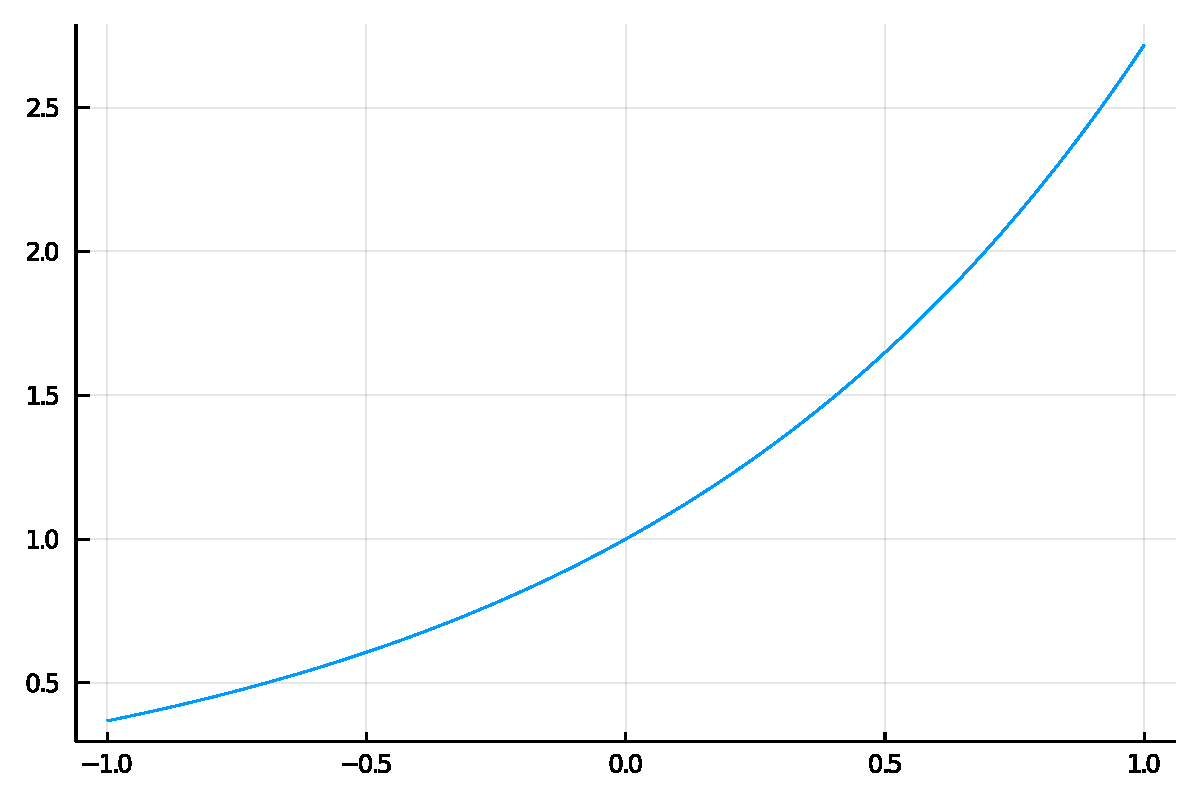
\includegraphics[width=0.8\linewidth]{C:/Users/mfaso/OneDrive/Documents/GitHub/M3M6AppliedComplexAnalysis/output/figures/Lecture20_9_1.pdf}}

It matches the "true" result:


\begin{lstlisting}
(*@\HLJLnf{u}@*)(*@\HLJLp{(}@*)(*@\HLJLnfB{0.1}@*)(*@\HLJLp{)}@*) (*@\HLJLp{,}@*) (*@\HLJLnf{exp}@*)(*@\HLJLp{(}@*)(*@\HLJLnfB{0.1}@*)(*@\HLJLp{)}@*)
\end{lstlisting}

\begin{lstlisting}
(1.1051709180756477, 1.1051709180756477)
\end{lstlisting}


Note we can incorporate right-hand sides as well, for example, to solve $u'(x) - u(x) = f(x)$, by expanding $f$ in its Chebyshev U series.

\subsubsection{Second-order constant coefficient equations}
This approach extends to second-order constant-coefficient equations by using ultraspherical polynomials.  Consider
\begin{align*}
u(-1) = 1,\: u(1) &= 0\\
u''(x) + u'(x)  + u(x) &= 0
\end{align*}
Evaluation works as in the first-order case. To handle second-derivatives, we need $C^{(2)}$ polynomials:
{\Large
\begin{lstlisting}
(*@\HLJLn{D\ensuremath{\_0}}@*) (*@\HLJLoB{=}@*) (*@\HLJLnf{Derivative}@*)(*@\HLJLp{()}@*) (*@\HLJLoB{:}@*) (*@\HLJLnf{Chebyshev}@*)(*@\HLJLp{()}@*) (*@\HLJLoB{\ensuremath{\rightarrow}}@*) (*@\HLJLnf{Ultraspherical}@*)(*@\HLJLp{(}@*)(*@\HLJLni{1}@*)(*@\HLJLp{)}@*)
(*@\HLJLn{D\ensuremath{\_1}}@*) (*@\HLJLoB{=}@*) (*@\HLJLnf{Derivative}@*)(*@\HLJLp{()}@*) (*@\HLJLoB{:}@*) (*@\HLJLnf{Ultraspherical}@*)(*@\HLJLp{(}@*)(*@\HLJLni{1}@*)(*@\HLJLp{)}@*) (*@\HLJLoB{\ensuremath{\rightarrow}}@*) (*@\HLJLnf{Ultraspherical}@*)(*@\HLJLp{(}@*)(*@\HLJLni{2}@*)(*@\HLJLp{)}@*)
(*@\HLJLn{D\ensuremath{\_1}}@*)(*@\HLJLoB{*}@*)(*@\HLJLn{D\ensuremath{\_0}}@*)  (*@\HLJLcs{{\#}}@*) (*@\HLJLcs{2}@*) (*@\HLJLcs{zeros}@*) (*@\HLJLcs{not}@*) (*@\HLJLcs{printed}@*) (*@\HLJLcs{in}@*) (*@\HLJLcs{(1,1)}@*) (*@\HLJLcs{and}@*) (*@\HLJLcs{(1,2)}@*) (*@\HLJLcs{entry}@*)
\end{lstlisting}
\begin{lstlisting}
ConcreteDerivative : Chebyshev() (*@\ensuremath{\to}@*) Ultraspherical(2)
 (*@\ensuremath{\cdot}@*)  (*@\ensuremath{\cdot}@*)  4.0   (*@\ensuremath{\cdot}@*)    (*@\ensuremath{\cdot}@*)     (*@\ensuremath{\cdot}@*)     (*@\ensuremath{\cdot}@*)     (*@\ensuremath{\cdot}@*)     (*@\ensuremath{\cdot}@*)     (*@\ensuremath{\cdot}@*)   (*@\ensuremath{\cdot}@*)
 (*@\ensuremath{\cdot}@*)  (*@\ensuremath{\cdot}@*)   (*@\ensuremath{\cdot}@*)   6.0   (*@\ensuremath{\cdot}@*)     (*@\ensuremath{\cdot}@*)     (*@\ensuremath{\cdot}@*)     (*@\ensuremath{\cdot}@*)     (*@\ensuremath{\cdot}@*)     (*@\ensuremath{\cdot}@*)   (*@\ensuremath{\cdot}@*)
 (*@\ensuremath{\cdot}@*)  (*@\ensuremath{\cdot}@*)   (*@\ensuremath{\cdot}@*)    (*@\ensuremath{\cdot}@*)   8.0    (*@\ensuremath{\cdot}@*)     (*@\ensuremath{\cdot}@*)     (*@\ensuremath{\cdot}@*)     (*@\ensuremath{\cdot}@*)     (*@\ensuremath{\cdot}@*)   (*@\ensuremath{\cdot}@*)
 (*@\ensuremath{\cdot}@*)  (*@\ensuremath{\cdot}@*)   (*@\ensuremath{\cdot}@*)    (*@\ensuremath{\cdot}@*)    (*@\ensuremath{\cdot}@*)   10.0    (*@\ensuremath{\cdot}@*)     (*@\ensuremath{\cdot}@*)     (*@\ensuremath{\cdot}@*)     (*@\ensuremath{\cdot}@*)   (*@\ensuremath{\cdot}@*)
 (*@\ensuremath{\cdot}@*)  (*@\ensuremath{\cdot}@*)   (*@\ensuremath{\cdot}@*)    (*@\ensuremath{\cdot}@*)    (*@\ensuremath{\cdot}@*)     (*@\ensuremath{\cdot}@*)   12.0    (*@\ensuremath{\cdot}@*)     (*@\ensuremath{\cdot}@*)     (*@\ensuremath{\cdot}@*)   (*@\ensuremath{\cdot}@*)
 (*@\ensuremath{\cdot}@*)  (*@\ensuremath{\cdot}@*)   (*@\ensuremath{\cdot}@*)    (*@\ensuremath{\cdot}@*)    (*@\ensuremath{\cdot}@*)     (*@\ensuremath{\cdot}@*)     (*@\ensuremath{\cdot}@*)   14.0    (*@\ensuremath{\cdot}@*)     (*@\ensuremath{\cdot}@*)   (*@\ensuremath{\cdot}@*)
 (*@\ensuremath{\cdot}@*)  (*@\ensuremath{\cdot}@*)   (*@\ensuremath{\cdot}@*)    (*@\ensuremath{\cdot}@*)    (*@\ensuremath{\cdot}@*)     (*@\ensuremath{\cdot}@*)     (*@\ensuremath{\cdot}@*)     (*@\ensuremath{\cdot}@*)   16.0    (*@\ensuremath{\cdot}@*)   (*@\ensuremath{\cdot}@*)
 (*@\ensuremath{\cdot}@*)  (*@\ensuremath{\cdot}@*)   (*@\ensuremath{\cdot}@*)    (*@\ensuremath{\cdot}@*)    (*@\ensuremath{\cdot}@*)     (*@\ensuremath{\cdot}@*)     (*@\ensuremath{\cdot}@*)     (*@\ensuremath{\cdot}@*)     (*@\ensuremath{\cdot}@*)   18.0  (*@\ensuremath{\cdot}@*)
 (*@\ensuremath{\cdot}@*)  (*@\ensuremath{\cdot}@*)   (*@\ensuremath{\cdot}@*)    (*@\ensuremath{\cdot}@*)    (*@\ensuremath{\cdot}@*)     (*@\ensuremath{\cdot}@*)     (*@\ensuremath{\cdot}@*)     (*@\ensuremath{\cdot}@*)     (*@\ensuremath{\cdot}@*)     (*@\ensuremath{\cdot}@*)   (*@\ensuremath{\ddots}@*)
 (*@\ensuremath{\cdot}@*)  (*@\ensuremath{\cdot}@*)   (*@\ensuremath{\cdot}@*)    (*@\ensuremath{\cdot}@*)    (*@\ensuremath{\cdot}@*)     (*@\ensuremath{\cdot}@*)     (*@\ensuremath{\cdot}@*)     (*@\ensuremath{\cdot}@*)     (*@\ensuremath{\cdot}@*)     (*@\ensuremath{\cdot}@*)   (*@\ensuremath{\ddots}@*)
 (*@\ensuremath{\cdot}@*)  (*@\ensuremath{\cdot}@*)   (*@\ensuremath{\cdot}@*)    (*@\ensuremath{\cdot}@*)    (*@\ensuremath{\cdot}@*)     (*@\ensuremath{\cdot}@*)     (*@\ensuremath{\cdot}@*)     (*@\ensuremath{\cdot}@*)     (*@\ensuremath{\cdot}@*)     (*@\ensuremath{\cdot}@*)   (*@\ensuremath{\ddots}@*)
\end{lstlisting}}


For the identity operator, we use two conversion operators:


\begin{lstlisting}
(*@\HLJLn{R{\_}TU}@*) (*@\HLJLoB{=}@*) (*@\HLJLn{I}@*) (*@\HLJLoB{:}@*) (*@\HLJLnf{Chebyshev}@*)(*@\HLJLp{()}@*) (*@\HLJLoB{\ensuremath{\rightarrow}}@*) (*@\HLJLnf{Ultraspherical}@*)(*@\HLJLp{(}@*)(*@\HLJLni{1}@*)(*@\HLJLp{)}@*)
(*@\HLJLn{R{\_}U2}@*) (*@\HLJLoB{=}@*) (*@\HLJLn{I}@*) (*@\HLJLoB{:}@*) (*@\HLJLnf{Ultraspherical}@*)(*@\HLJLp{(}@*)(*@\HLJLni{1}@*)(*@\HLJLp{)}@*) (*@\HLJLoB{\ensuremath{\rightarrow}}@*) (*@\HLJLnf{Ultraspherical}@*)(*@\HLJLp{(}@*)(*@\HLJLni{2}@*)(*@\HLJLp{)}@*)
(*@\HLJLn{R{\_}T2}@*) (*@\HLJLoB{=}@*) (*@\HLJLn{R{\_}U2}@*)(*@\HLJLoB{*}@*)(*@\HLJLn{R{\_}TU}@*)
\end{lstlisting}
{\Large
\begin{lstlisting}
TimesOperator : Chebyshev() (*@\ensuremath{\to}@*) Ultraspherical(2)
 1.0  0.0   -0.6666666666666666    0.0    (*@\ensuremath{\dots}@*)    (*@\ensuremath{\cdot}@*)                     (*@\ensuremath{\cdot}@*)     
 (*@\ensuremath{\cdot}@*)
  (*@\ensuremath{\cdot}@*)   0.25   0.0                  -0.375       (*@\ensuremath{\cdot}@*)                     (*@\ensuremath{\cdot}@*)     
 (*@\ensuremath{\cdot}@*)
  (*@\ensuremath{\cdot}@*)    (*@\ensuremath{\cdot}@*)     0.16666666666666666   0.0         (*@\ensuremath{\cdot}@*)                     (*@\ensuremath{\cdot}@*)     
 (*@\ensuremath{\cdot}@*)
  (*@\ensuremath{\cdot}@*)    (*@\ensuremath{\cdot}@*)      (*@\ensuremath{\cdot}@*)                    0.125       (*@\ensuremath{\cdot}@*)                     (*@\ensuremath{\cdot}@*)     
 (*@\ensuremath{\cdot}@*)
  (*@\ensuremath{\cdot}@*)    (*@\ensuremath{\cdot}@*)      (*@\ensuremath{\cdot}@*)                     (*@\ensuremath{\cdot}@*)         0.07142857142857142    (*@\ensuremath{\cdot}@*)     
 (*@\ensuremath{\cdot}@*)
  (*@\ensuremath{\cdot}@*)    (*@\ensuremath{\cdot}@*)      (*@\ensuremath{\cdot}@*)                     (*@\ensuremath{\cdot}@*)     (*@\ensuremath{\dots}@*)   0.0                   0.0625 
 (*@\ensuremath{\cdot}@*)
  (*@\ensuremath{\cdot}@*)    (*@\ensuremath{\cdot}@*)      (*@\ensuremath{\cdot}@*)                     (*@\ensuremath{\cdot}@*)        -0.12698412698412698   0.0    
 (*@\ensuremath{\ddots}@*)
  (*@\ensuremath{\cdot}@*)    (*@\ensuremath{\cdot}@*)      (*@\ensuremath{\cdot}@*)                     (*@\ensuremath{\cdot}@*)         0.0                  -0.1125 
 (*@\ensuremath{\ddots}@*)
  (*@\ensuremath{\cdot}@*)    (*@\ensuremath{\cdot}@*)      (*@\ensuremath{\cdot}@*)                     (*@\ensuremath{\cdot}@*)         0.05555555555555555   0.0    
 (*@\ensuremath{\ddots}@*)
  (*@\ensuremath{\cdot}@*)    (*@\ensuremath{\cdot}@*)      (*@\ensuremath{\cdot}@*)                     (*@\ensuremath{\cdot}@*)          (*@\ensuremath{\cdot}@*)                    0.05   
 (*@\ensuremath{\ddots}@*)
  (*@\ensuremath{\cdot}@*)    (*@\ensuremath{\cdot}@*)      (*@\ensuremath{\cdot}@*)                     (*@\ensuremath{\cdot}@*)     (*@\ensuremath{\dots}@*)    (*@\ensuremath{\cdot}@*)                     (*@\ensuremath{\cdot}@*)     
 (*@\ensuremath{\ddots}@*)
\end{lstlisting}}


And for the first derivative, we use a derivative and then a conversion:


\begin{lstlisting}
(*@\HLJLn{R{\_}U2}@*)(*@\HLJLoB{*}@*)(*@\HLJLn{D\ensuremath{\_0}}@*)  (*@\HLJLcs{{\#}}@*) (*@\HLJLcs{or}@*) (*@\HLJLcs{could}@*) (*@\HLJLcs{have}@*) (*@\HLJLcs{been}@*) (*@\HLJLcs{D\ensuremath{\_1}*R\ensuremath{\_}TU}@*)
\end{lstlisting}

\begin{lstlisting}
TimesOperator : Chebyshev() (*@\ensuremath{\to}@*) Ultraspherical(2)
 (*@\ensuremath{\cdot}@*)  1.0  0.0  -1.0    (*@\ensuremath{\cdot}@*)     (*@\ensuremath{\cdot}@*)     (*@\ensuremath{\cdot}@*)     (*@\ensuremath{\cdot}@*)     (*@\ensuremath{\cdot}@*)     (*@\ensuremath{\cdot}@*)   (*@\ensuremath{\cdot}@*)
 (*@\ensuremath{\cdot}@*)   (*@\ensuremath{\cdot}@*)   1.0   0.0  -1.0    (*@\ensuremath{\cdot}@*)     (*@\ensuremath{\cdot}@*)     (*@\ensuremath{\cdot}@*)     (*@\ensuremath{\cdot}@*)     (*@\ensuremath{\cdot}@*)   (*@\ensuremath{\cdot}@*)
 (*@\ensuremath{\cdot}@*)   (*@\ensuremath{\cdot}@*)    (*@\ensuremath{\cdot}@*)    1.0   0.0  -1.0    (*@\ensuremath{\cdot}@*)     (*@\ensuremath{\cdot}@*)     (*@\ensuremath{\cdot}@*)     (*@\ensuremath{\cdot}@*)   (*@\ensuremath{\cdot}@*)
 (*@\ensuremath{\cdot}@*)   (*@\ensuremath{\cdot}@*)    (*@\ensuremath{\cdot}@*)     (*@\ensuremath{\cdot}@*)    1.0   0.0  -1.0    (*@\ensuremath{\cdot}@*)     (*@\ensuremath{\cdot}@*)     (*@\ensuremath{\cdot}@*)   (*@\ensuremath{\cdot}@*)
 (*@\ensuremath{\cdot}@*)   (*@\ensuremath{\cdot}@*)    (*@\ensuremath{\cdot}@*)     (*@\ensuremath{\cdot}@*)     (*@\ensuremath{\cdot}@*)    1.0   0.0  -1.0    (*@\ensuremath{\cdot}@*)     (*@\ensuremath{\cdot}@*)   (*@\ensuremath{\cdot}@*)
 (*@\ensuremath{\cdot}@*)   (*@\ensuremath{\cdot}@*)    (*@\ensuremath{\cdot}@*)     (*@\ensuremath{\cdot}@*)     (*@\ensuremath{\cdot}@*)     (*@\ensuremath{\cdot}@*)    1.0   0.0  -1.0    (*@\ensuremath{\cdot}@*)   (*@\ensuremath{\cdot}@*)
 (*@\ensuremath{\cdot}@*)   (*@\ensuremath{\cdot}@*)    (*@\ensuremath{\cdot}@*)     (*@\ensuremath{\cdot}@*)     (*@\ensuremath{\cdot}@*)     (*@\ensuremath{\cdot}@*)     (*@\ensuremath{\cdot}@*)    1.0   0.0  -1.0  (*@\ensuremath{\cdot}@*)
 (*@\ensuremath{\cdot}@*)   (*@\ensuremath{\cdot}@*)    (*@\ensuremath{\cdot}@*)     (*@\ensuremath{\cdot}@*)     (*@\ensuremath{\cdot}@*)     (*@\ensuremath{\cdot}@*)     (*@\ensuremath{\cdot}@*)     (*@\ensuremath{\cdot}@*)    1.0   0.0  (*@\ensuremath{\ddots}@*)
 (*@\ensuremath{\cdot}@*)   (*@\ensuremath{\cdot}@*)    (*@\ensuremath{\cdot}@*)     (*@\ensuremath{\cdot}@*)     (*@\ensuremath{\cdot}@*)     (*@\ensuremath{\cdot}@*)     (*@\ensuremath{\cdot}@*)     (*@\ensuremath{\cdot}@*)     (*@\ensuremath{\cdot}@*)    1.0  (*@\ensuremath{\ddots}@*)
 (*@\ensuremath{\cdot}@*)   (*@\ensuremath{\cdot}@*)    (*@\ensuremath{\cdot}@*)     (*@\ensuremath{\cdot}@*)     (*@\ensuremath{\cdot}@*)     (*@\ensuremath{\cdot}@*)     (*@\ensuremath{\cdot}@*)     (*@\ensuremath{\cdot}@*)     (*@\ensuremath{\cdot}@*)     (*@\ensuremath{\cdot}@*)   (*@\ensuremath{\ddots}@*)
 (*@\ensuremath{\cdot}@*)   (*@\ensuremath{\cdot}@*)    (*@\ensuremath{\cdot}@*)     (*@\ensuremath{\cdot}@*)     (*@\ensuremath{\cdot}@*)     (*@\ensuremath{\cdot}@*)     (*@\ensuremath{\cdot}@*)     (*@\ensuremath{\cdot}@*)     (*@\ensuremath{\cdot}@*)     (*@\ensuremath{\cdot}@*)   (*@\ensuremath{\ddots}@*)
\end{lstlisting}


Putting everything together we get:


\begin{lstlisting}
(*@\HLJLn{B\ensuremath{\_-}\ensuremath{\_1}}@*) (*@\HLJLoB{=}@*) (*@\HLJLnf{Evaluation}@*)(*@\HLJLp{(}@*)(*@\HLJLoB{-}@*)(*@\HLJLni{1}@*)(*@\HLJLp{)}@*) (*@\HLJLoB{:}@*) (*@\HLJLnf{Chebyshev}@*)(*@\HLJLp{()}@*)
(*@\HLJLn{B\ensuremath{\_1}}@*) (*@\HLJLoB{=}@*) (*@\HLJLnf{Evaluation}@*)(*@\HLJLp{(}@*)(*@\HLJLni{1}@*)(*@\HLJLp{)}@*) (*@\HLJLoB{:}@*) (*@\HLJLnf{Chebyshev}@*)(*@\HLJLp{()}@*)
(*@\HLJLcs{{\#}}@*) (*@\HLJLcs{u(-1)}@*)
(*@\HLJLcs{{\#}}@*) (*@\HLJLcs{u(1)}@*)
(*@\HLJLcs{{\#}}@*) (*@\HLJLcs{u{\textquotesingle}{\textquotesingle}}@*) (*@\HLJLcs{+}@*) (*@\HLJLcs{u{\textquotesingle}}@*) (*@\HLJLcs{+u}@*)
(*@\HLJLn{L}@*) (*@\HLJLoB{=}@*) (*@\HLJLp{[}@*)(*@\HLJLn{B\ensuremath{\_-}\ensuremath{\_1}}@*)(*@\HLJLp{;}@*)
     (*@\HLJLn{B\ensuremath{\_1}}@*)(*@\HLJLp{;}@*)
     (*@\HLJLn{D\ensuremath{\_1}}@*)(*@\HLJLoB{*}@*)(*@\HLJLn{D\ensuremath{\_0}}@*) (*@\HLJLoB{+}@*) (*@\HLJLn{R{\_}U2}@*)(*@\HLJLoB{*}@*)(*@\HLJLn{D\ensuremath{\_0}}@*) (*@\HLJLoB{+}@*) (*@\HLJLn{R{\_}U2}@*)(*@\HLJLoB{*}@*)(*@\HLJLn{R{\_}TU}@*)(*@\HLJLp{]}@*)
(*@\HLJLn{u}@*) (*@\HLJLoB{=}@*) (*@\HLJLn{L}@*) (*@\HLJLoB{{\textbackslash}}@*) (*@\HLJLp{[}@*)(*@\HLJLnfB{1.0}@*)(*@\HLJLp{,}@*)(*@\HLJLnfB{0.0}@*)(*@\HLJLp{,}@*)(*@\HLJLnfB{0.0}@*)(*@\HLJLp{]}@*)
(*@\HLJLnf{plot}@*)(*@\HLJLp{(}@*)(*@\HLJLn{u}@*)(*@\HLJLp{)}@*)
\end{lstlisting}

\cent{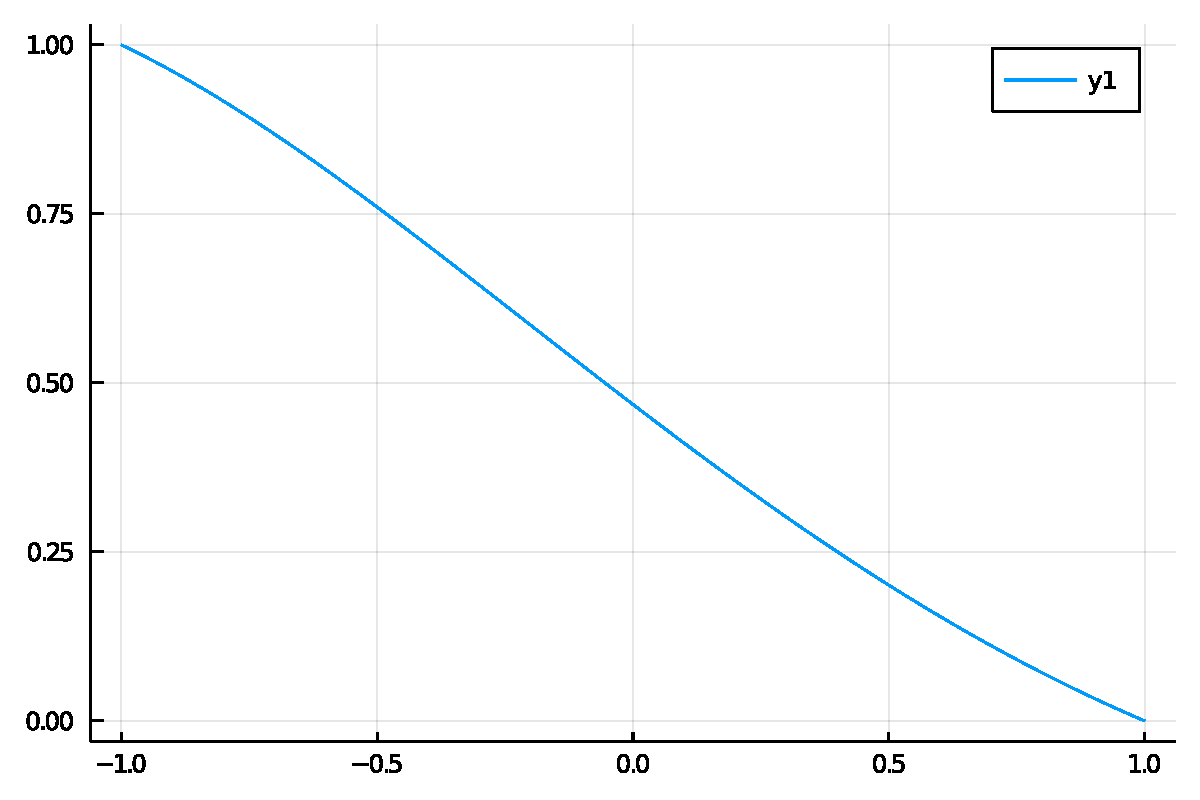
\includegraphics[width=0.75\linewidth]{C:/Users/mfaso/OneDrive/Documents/GitHub/M3M6AppliedComplexAnalysis/output/figures/Lecture20_14_1.pdf}}

\subsubsection{Variable coefficients}
Consider the Airy ODE
\begin{align*}
u(-1) &= 1\\
u(1) &= 0\\
u''(x) - xu(x) &= 0
\end{align*}
to handle this, we need only use the Jacobi operator to represent multiplication by $x$:


\begin{lstlisting}
(*@\HLJLn{x}@*) (*@\HLJLoB{=}@*) (*@\HLJLnf{Fun}@*)(*@\HLJLp{()}@*)
(*@\HLJLn{X}@*) (*@\HLJLoB{=}@*) (*@\HLJLnf{Multiplication}@*)(*@\HLJLp{(}@*)(*@\HLJLn{x}@*)(*@\HLJLp{)}@*) (*@\HLJLoB{:}@*) (*@\HLJLnf{Chebyshev}@*)(*@\HLJLp{()}@*) (*@\HLJLoB{\ensuremath{\rightarrow}}@*) (*@\HLJLnf{Chebyshev}@*)(*@\HLJLp{()}@*)  (*@\HLJLcs{{\#}}@*) (*@\HLJLcs{transpose}@*) (*@\HLJLcs{of}@*) (*@\HLJLcs{the}@*) (*@\HLJLcs{Jacobi}@*) (*@\HLJLcs{operator}@*)
\end{lstlisting}

\begin{lstlisting}
ConcreteMultiplication : Chebyshev() (*@\ensuremath{\to}@*) Chebyshev()
 0.0  0.5   (*@\ensuremath{\cdot}@*)    (*@\ensuremath{\cdot}@*)    (*@\ensuremath{\cdot}@*)    (*@\ensuremath{\cdot}@*)    (*@\ensuremath{\cdot}@*)    (*@\ensuremath{\cdot}@*)    (*@\ensuremath{\cdot}@*)    (*@\ensuremath{\cdot}@*)   (*@\ensuremath{\cdot}@*)
 1.0  0.0  0.5   (*@\ensuremath{\cdot}@*)    (*@\ensuremath{\cdot}@*)    (*@\ensuremath{\cdot}@*)    (*@\ensuremath{\cdot}@*)    (*@\ensuremath{\cdot}@*)    (*@\ensuremath{\cdot}@*)    (*@\ensuremath{\cdot}@*)   (*@\ensuremath{\cdot}@*)
  (*@\ensuremath{\cdot}@*)   0.5  0.0  0.5   (*@\ensuremath{\cdot}@*)    (*@\ensuremath{\cdot}@*)    (*@\ensuremath{\cdot}@*)    (*@\ensuremath{\cdot}@*)    (*@\ensuremath{\cdot}@*)    (*@\ensuremath{\cdot}@*)   (*@\ensuremath{\cdot}@*)
  (*@\ensuremath{\cdot}@*)    (*@\ensuremath{\cdot}@*)   0.5  0.0  0.5   (*@\ensuremath{\cdot}@*)    (*@\ensuremath{\cdot}@*)    (*@\ensuremath{\cdot}@*)    (*@\ensuremath{\cdot}@*)    (*@\ensuremath{\cdot}@*)   (*@\ensuremath{\cdot}@*)
  (*@\ensuremath{\cdot}@*)    (*@\ensuremath{\cdot}@*)    (*@\ensuremath{\cdot}@*)   0.5  0.0  0.5   (*@\ensuremath{\cdot}@*)    (*@\ensuremath{\cdot}@*)    (*@\ensuremath{\cdot}@*)    (*@\ensuremath{\cdot}@*)   (*@\ensuremath{\cdot}@*)
  (*@\ensuremath{\cdot}@*)    (*@\ensuremath{\cdot}@*)    (*@\ensuremath{\cdot}@*)    (*@\ensuremath{\cdot}@*)   0.5  0.0  0.5   (*@\ensuremath{\cdot}@*)    (*@\ensuremath{\cdot}@*)    (*@\ensuremath{\cdot}@*)   (*@\ensuremath{\cdot}@*)
  (*@\ensuremath{\cdot}@*)    (*@\ensuremath{\cdot}@*)    (*@\ensuremath{\cdot}@*)    (*@\ensuremath{\cdot}@*)    (*@\ensuremath{\cdot}@*)   0.5  0.0  0.5   (*@\ensuremath{\cdot}@*)    (*@\ensuremath{\cdot}@*)   (*@\ensuremath{\cdot}@*)
  (*@\ensuremath{\cdot}@*)    (*@\ensuremath{\cdot}@*)    (*@\ensuremath{\cdot}@*)    (*@\ensuremath{\cdot}@*)    (*@\ensuremath{\cdot}@*)    (*@\ensuremath{\cdot}@*)   0.5  0.0  0.5   (*@\ensuremath{\cdot}@*)   (*@\ensuremath{\cdot}@*)
  (*@\ensuremath{\cdot}@*)    (*@\ensuremath{\cdot}@*)    (*@\ensuremath{\cdot}@*)    (*@\ensuremath{\cdot}@*)    (*@\ensuremath{\cdot}@*)    (*@\ensuremath{\cdot}@*)    (*@\ensuremath{\cdot}@*)   0.5  0.0  0.5  (*@\ensuremath{\cdot}@*)
  (*@\ensuremath{\cdot}@*)    (*@\ensuremath{\cdot}@*)    (*@\ensuremath{\cdot}@*)    (*@\ensuremath{\cdot}@*)    (*@\ensuremath{\cdot}@*)    (*@\ensuremath{\cdot}@*)    (*@\ensuremath{\cdot}@*)    (*@\ensuremath{\cdot}@*)   0.5  0.0  (*@\ensuremath{\ddots}@*)
  (*@\ensuremath{\cdot}@*)    (*@\ensuremath{\cdot}@*)    (*@\ensuremath{\cdot}@*)    (*@\ensuremath{\cdot}@*)    (*@\ensuremath{\cdot}@*)    (*@\ensuremath{\cdot}@*)    (*@\ensuremath{\cdot}@*)    (*@\ensuremath{\cdot}@*)    (*@\ensuremath{\cdot}@*)    (*@\ensuremath{\ddots}@*)   (*@\ensuremath{\ddots}@*)
\end{lstlisting}


We set up the system as follows:


\begin{lstlisting}
(*@\HLJLn{L}@*) (*@\HLJLoB{=}@*) (*@\HLJLp{[}@*)(*@\HLJLn{B\ensuremath{\_-}\ensuremath{\_1}}@*)(*@\HLJLp{;}@*)   (*@\HLJLcs{{\#}}@*) (*@\HLJLcs{u(-1)}@*)
     (*@\HLJLn{B\ensuremath{\_1}}@*) (*@\HLJLp{;}@*)   (*@\HLJLcs{{\#}}@*) (*@\HLJLcs{u(1)}@*)
     (*@\HLJLn{D\ensuremath{\_1}}@*)(*@\HLJLoB{*}@*)(*@\HLJLn{D\ensuremath{\_0}}@*) (*@\HLJLoB{-}@*) (*@\HLJLn{R{\_}U2}@*)(*@\HLJLoB{*}@*)(*@\HLJLn{R{\_}TU}@*)(*@\HLJLoB{*}@*)(*@\HLJLn{X}@*)(*@\HLJLp{]}@*)   (*@\HLJLcs{{\#}}@*) (*@\HLJLcs{u{\textquotesingle}{\textquotesingle}}@*) (*@\HLJLcs{-}@*) (*@\HLJLcs{x*u}@*)
(*@\HLJLn{u}@*) (*@\HLJLoB{=}@*) (*@\HLJLn{L}@*) (*@\HLJLoB{{\textbackslash}}@*) (*@\HLJLp{[}@*)(*@\HLJLnfB{1.0}@*)(*@\HLJLp{;}@*)(*@\HLJLnfB{0.0}@*)(*@\HLJLp{;}@*)(*@\HLJLnfB{0.0}@*)(*@\HLJLp{]}@*)
(*@\HLJLnf{plot}@*)(*@\HLJLp{(}@*)(*@\HLJLn{u}@*)(*@\HLJLp{;}@*) (*@\HLJLn{legend}@*)(*@\HLJLoB{=}@*)(*@\HLJLkc{false}@*)(*@\HLJLp{)}@*)
\end{lstlisting}

\cent{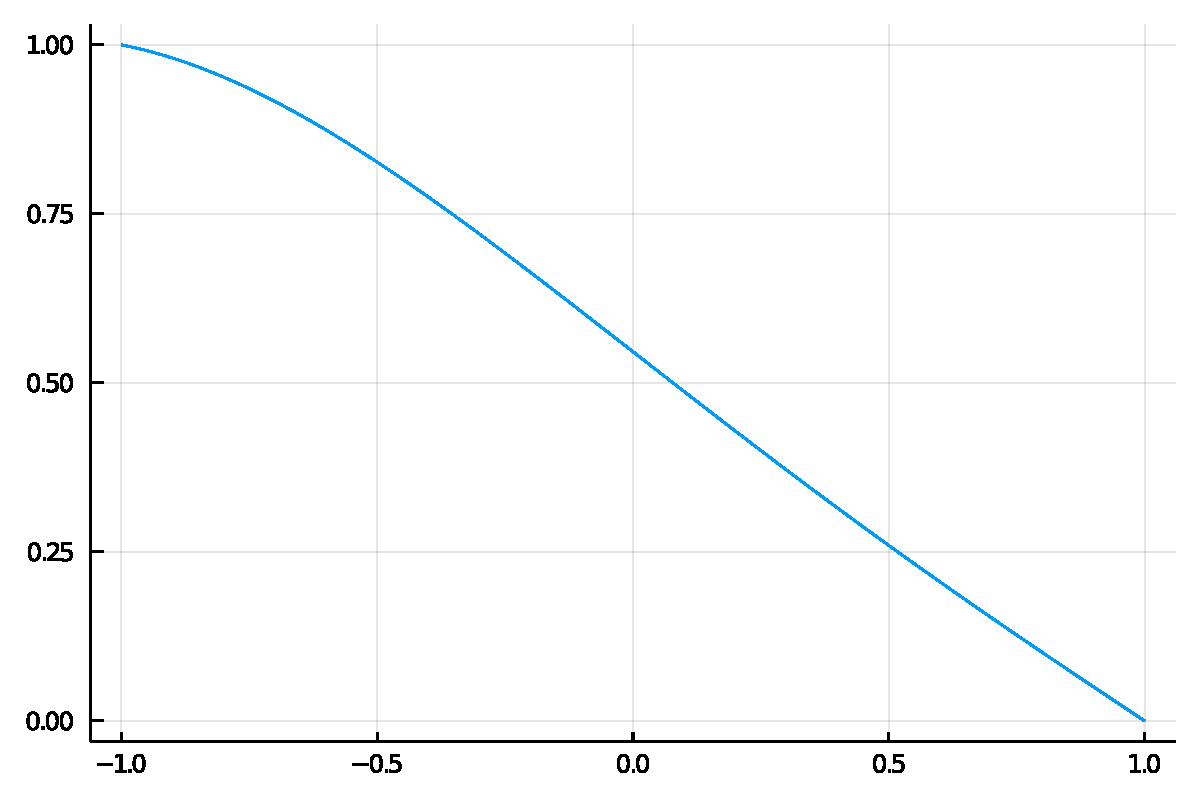
\includegraphics[width=0.8\linewidth]{C:/Users/mfaso/OneDrive/Documents/GitHub/M3M6AppliedComplexAnalysis/output/figures/Lecture20_16_1.pdf}}

If we introduce a small parameter, that is, solve
\begin{align*}
u(-1) = 1, \: 
u(1) &= 0\\
\epsilon u''(x) - xu(x) &= 0
\end{align*}
we can see it's pretty hard to compute solutions:


\begin{lstlisting}
(*@\HLJLn{\ensuremath{\varepsilon}}@*) (*@\HLJLoB{=}@*) (*@\HLJLnfB{1E-6}@*)
(*@\HLJLn{L}@*) (*@\HLJLoB{=}@*) (*@\HLJLp{[}@*)(*@\HLJLn{B\ensuremath{\_-}\ensuremath{\_1}}@*)(*@\HLJLp{;}@*)
     (*@\HLJLn{B\ensuremath{\_1}}@*) (*@\HLJLp{;}@*)
     (*@\HLJLn{\ensuremath{\varepsilon}}@*)(*@\HLJLoB{*}@*)(*@\HLJLn{D\ensuremath{\_1}}@*)(*@\HLJLoB{*}@*)(*@\HLJLn{D\ensuremath{\_0}}@*) (*@\HLJLoB{-}@*) (*@\HLJLn{R{\_}U2}@*)(*@\HLJLoB{*}@*)(*@\HLJLn{R{\_}TU}@*)(*@\HLJLoB{*}@*)(*@\HLJLn{X}@*)(*@\HLJLp{]}@*)
(*@\HLJLn{u}@*) (*@\HLJLoB{=}@*) (*@\HLJLn{L}@*) (*@\HLJLoB{{\textbackslash}}@*) (*@\HLJLp{[}@*)(*@\HLJLnfB{1.0}@*)(*@\HLJLp{;}@*)(*@\HLJLnfB{0.0}@*)(*@\HLJLp{;}@*)(*@\HLJLnfB{0.0}@*)(*@\HLJLp{]}@*)
(*@\HLJLnf{plot}@*)(*@\HLJLp{(}@*)(*@\HLJLn{u}@*)(*@\HLJLp{;}@*) (*@\HLJLn{legend}@*)(*@\HLJLoB{=}@*)(*@\HLJLkc{false}@*)(*@\HLJLp{)}@*)
\end{lstlisting}
\cent{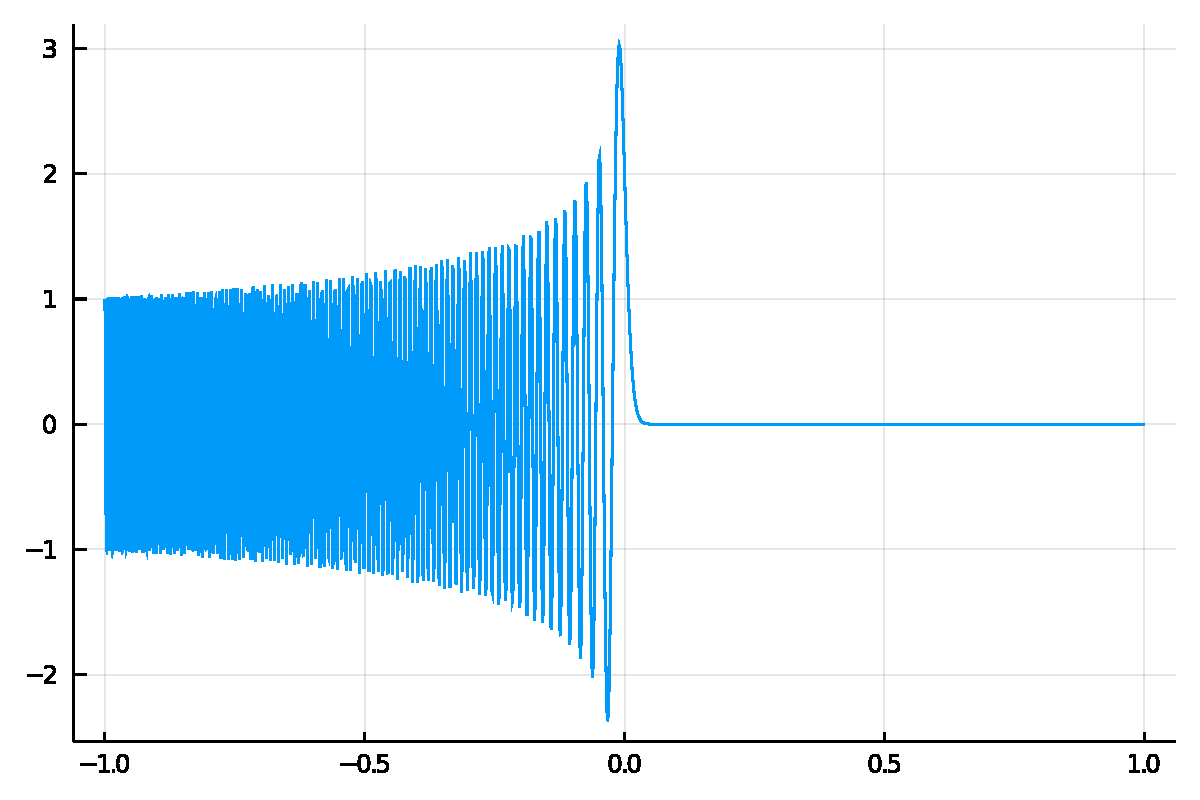
\includegraphics[width=0.55\linewidth]{C:/Users/mfaso/OneDrive/Documents/GitHub/M3M6AppliedComplexAnalysis/output/figures/Lecture20_17_1.pdf}}

Because of the banded structure, this can be solved fast:


\begin{lstlisting}
(*@\HLJLn{\ensuremath{\varepsilon}}@*) (*@\HLJLoB{=}@*) (*@\HLJLnfB{1E-10}@*)
(*@\HLJLn{L}@*) (*@\HLJLoB{=}@*) (*@\HLJLp{[}@*)(*@\HLJLn{B\ensuremath{\_-}\ensuremath{\_1}}@*)(*@\HLJLp{;}@*)
     (*@\HLJLn{B\ensuremath{\_1}}@*) (*@\HLJLp{;}@*)
     (*@\HLJLn{\ensuremath{\varepsilon}}@*)(*@\HLJLoB{*}@*)(*@\HLJLn{D\ensuremath{\_1}}@*)(*@\HLJLoB{*}@*)(*@\HLJLn{D\ensuremath{\_0}}@*) (*@\HLJLoB{-}@*) (*@\HLJLn{R{\_}U2}@*)(*@\HLJLoB{*}@*)(*@\HLJLn{R{\_}TU}@*)(*@\HLJLoB{*}@*)(*@\HLJLn{X}@*)(*@\HLJLp{]}@*)

(*@\HLJLnd{@time}@*) (*@\HLJLn{u}@*) (*@\HLJLoB{=}@*) (*@\HLJLn{L}@*) (*@\HLJLoB{{\textbackslash}}@*) (*@\HLJLp{[}@*)(*@\HLJLnfB{1.0}@*)(*@\HLJLp{;}@*)(*@\HLJLnfB{0.0}@*)(*@\HLJLp{;}@*)(*@\HLJLnfB{0.0}@*)(*@\HLJLp{]}@*)
(*@\HLJLnd{@show}@*) (*@\HLJLnf{ncoefficients}@*)(*@\HLJLp{(}@*)(*@\HLJLn{u}@*)(*@\HLJLp{);}@*)
\end{lstlisting}

\begin{lstlisting}
3.457937 seconds (10.63 M allocations: 260.175 MiB, 19.17(*@{{\%}}@*) gc time)
ncoefficients(u) = 62496
\end{lstlisting}


To handle other variable coefficients, first consider a polynomial $p(x)$. If Multiplication by $x$ is represented by multiplying the coefficients by $J^\top$, then multiplication by $p$ is represented by $p(J^\top)$:


\begin{lstlisting}
(*@\HLJLn{M}@*) (*@\HLJLoB{=}@*) (*@\HLJLoB{-}@*)(*@\HLJLn{I}@*) (*@\HLJLoB{+}@*) (*@\HLJLn{X}@*) (*@\HLJLoB{+}@*) (*@\HLJLp{(}@*)(*@\HLJLn{X}@*)(*@\HLJLp{)}@*)(*@\HLJLoB{{\textasciicircum}}@*)(*@\HLJLni{2}@*)  (*@\HLJLcs{{\#}}@*) (*@\HLJLcs{represents}@*) (*@\HLJLcs{-1+x+x{\textasciicircum}2}@*)

(*@\HLJLn{\ensuremath{\varepsilon}}@*) (*@\HLJLoB{=}@*) (*@\HLJLnfB{1E-6}@*)
(*@\HLJLn{L}@*) (*@\HLJLoB{=}@*) (*@\HLJLp{[}@*)(*@\HLJLn{B\ensuremath{\_-}\ensuremath{\_1}}@*)(*@\HLJLp{;}@*)
     (*@\HLJLn{B\ensuremath{\_1}}@*) (*@\HLJLp{;}@*)
     (*@\HLJLn{\ensuremath{\varepsilon}}@*)(*@\HLJLoB{*}@*)(*@\HLJLn{D\ensuremath{\_1}}@*)(*@\HLJLoB{*}@*)(*@\HLJLn{D\ensuremath{\_0}}@*) (*@\HLJLoB{-}@*) (*@\HLJLn{R{\_}U2}@*)(*@\HLJLoB{*}@*)(*@\HLJLn{R{\_}TU}@*)(*@\HLJLoB{*}@*)(*@\HLJLn{M}@*)(*@\HLJLp{]}@*)

(*@\HLJLnd{@time}@*) (*@\HLJLn{u}@*) (*@\HLJLoB{=}@*) (*@\HLJLn{L}@*) (*@\HLJLoB{{\textbackslash}}@*) (*@\HLJLp{[}@*)(*@\HLJLnfB{1.0}@*)(*@\HLJLp{;}@*)(*@\HLJLnfB{0.0}@*)(*@\HLJLp{;}@*)(*@\HLJLnfB{0.0}@*)(*@\HLJLp{]}@*)

(*@\HLJLnd{@show}@*) (*@\HLJLn{\ensuremath{\varepsilon}}@*)(*@\HLJLoB{*}@*)(*@\HLJLn{u}@*)(*@\HLJLoB{{\textquotesingle}{\textquotesingle}}@*)(*@\HLJLp{(}@*)(*@\HLJLnfB{0.1}@*)(*@\HLJLp{)}@*) (*@\HLJLoB{-}@*) (*@\HLJLp{(}@*)(*@\HLJLoB{-}@*)(*@\HLJLni{1}@*)(*@\HLJLoB{+}@*)(*@\HLJLnfB{0.1}@*)(*@\HLJLoB{+}@*)(*@\HLJLnfB{0.1}@*)(*@\HLJLoB{{\textasciicircum}}@*)(*@\HLJLni{2}@*)(*@\HLJLp{)}@*)(*@\HLJLoB{*}@*)(*@\HLJLnf{u}@*)(*@\HLJLp{(}@*)(*@\HLJLnfB{0.1}@*)(*@\HLJLp{)}@*)
(*@\HLJLnf{plot}@*)(*@\HLJLp{(}@*)(*@\HLJLn{u}@*)(*@\HLJLp{)}@*)
\end{lstlisting}

\begin{lstlisting}
0.109666 seconds (229.04 k allocations: 5.980 MiB)
(*@\ensuremath{\upepsilon}@*) * ((u(*@{{\textquotesingle}}@*))(*@{{\textquotesingle}}@*))(0.1) - (-1 + 0.1 + 0.1 (*@{{\textasciicircum}}@*) 2) * u(0.1) = -1.3572476476042539e-14
\end{lstlisting}

%\begin{lstlisting}
%(*@\ensuremath{\upepsilon}@*) * ((u(*@{{\textquotesingle}}@*))(*@{{\textquotesingle}}@*))(0.1) - (-1 + 0.1 + 0.1 (*@{{\textasciicircum}}@*) 2) * u(0.1) = -1.3572476476042539e-14
%\end{lstlisting}

\cent{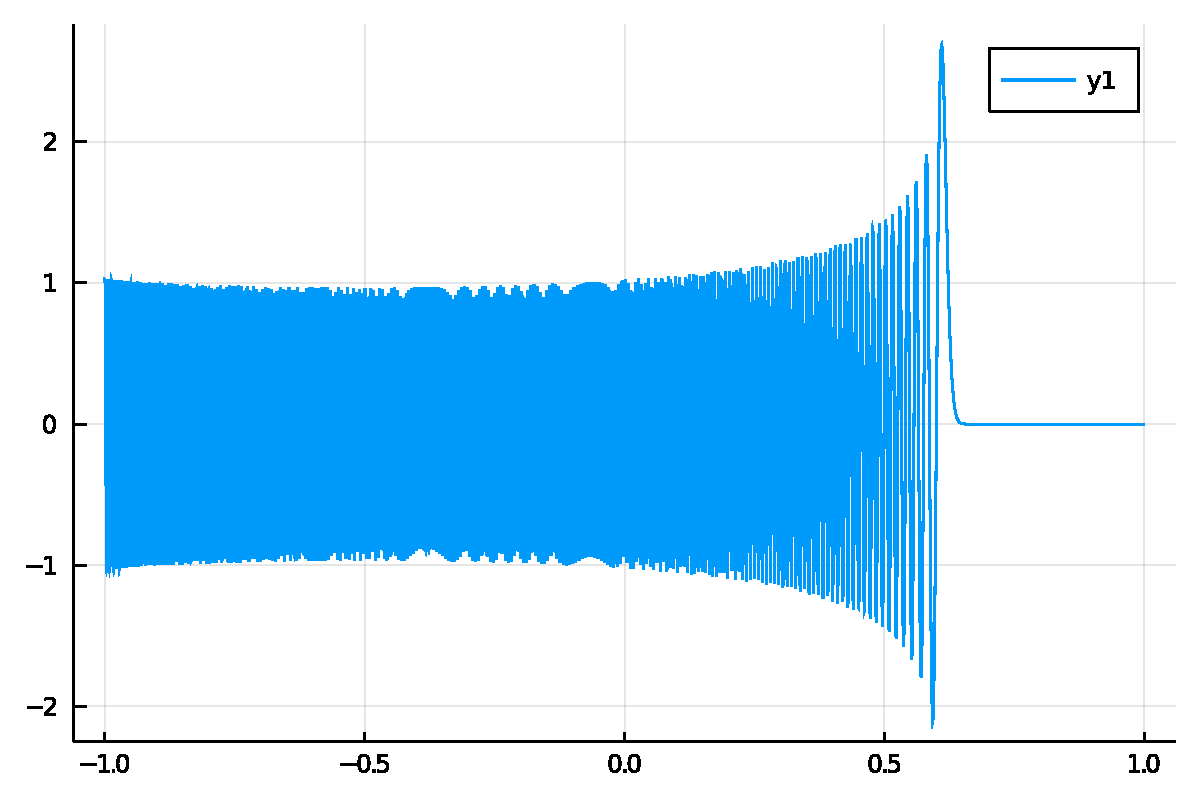
\includegraphics[width=0.8\linewidth]{C:/Users/mfaso/OneDrive/Documents/GitHub/M3M6AppliedComplexAnalysis/output/figures/Lecture20_19_1.pdf}}

For other smooth functions, we first approximate in a polynomial basis,  and without loss of generality we use Chebyshev T basis. For example, consider


\begin{align*}
u(-1) &= 1\\
u(1) &= 0\\
\epsilon u''(x) - \E^x u(x) &= 0
\end{align*}
where

\[
\E^x  \approx p(x) = \sum_{k=0}^{m-1} p_k T_k(x)
\]
Evaluating at a point $x$, recall Clenshaw's algorithm:


\begin{align*}
\gamma_{n-1} &= 2p_{n-1} \\
\gamma_{n-2} &= 2p_{n-2} + 2x \gamma_{n-1} \\
\gamma_{n-3} &= 2 p_{n-3} + 2x \gamma_{n-2} - \gamma_{n-1} \\
& \vdots \\
\gamma_1 &= p_1 + x \gamma_2 - \half \gamma_3 \\
p(x) = \gamma_0 &= p_0 + x \gamma_1 - \half \gamma_2
\end{align*}
If multiplication by $x$ becomes $J^\top$, then multiplication by $p(x)$ becomes $p(J^\top)$, and hence we calculate:


\begin{align*}
\Gamma_{n-1} &= 2p_{n-1}I \\
\Gamma_{n-2} &= 2p_{n-2}I + 2J^\top \Gamma_{n-1} \\
\Gamma_{n-3} &= 2 p_{n-3}I + 2J^\top \Gamma_{n-2} - \Gamma_{n-1} \\
& \vdots \\
\Gamma_1 &= p_1I + J^\top \Gamma_2 - \half \Gamma_3 \\
p(J^\top) = \Gamma_0 &= p_0 + x \Gamma_1 - \half \Gamma_2
\end{align*}
Here is an example:


\begin{lstlisting}
(*@\HLJLn{p}@*) (*@\HLJLoB{=}@*) (*@\HLJLnf{Fun}@*)(*@\HLJLp{(}@*)(*@\HLJLn{exp}@*)(*@\HLJLp{,}@*) (*@\HLJLnf{Chebyshev}@*)(*@\HLJLp{())}@*) (*@\HLJLcs{{\#}}@*) (*@\HLJLcs{polynomial}@*) (*@\HLJLcs{approximation}@*) (*@\HLJLcs{to}@*) (*@\HLJLcs{exp(x)}@*)
(*@\HLJLn{M}@*) (*@\HLJLoB{=}@*) (*@\HLJLnf{Multiplication}@*)(*@\HLJLp{(}@*)(*@\HLJLn{p}@*)(*@\HLJLp{)}@*) (*@\HLJLoB{:}@*) (*@\HLJLnf{Chebyshev}@*)(*@\HLJLp{()}@*) (*@\HLJLcs{{\#}}@*) (*@\HLJLcs{constructed}@*) (*@\HLJLcs{using}@*) (*@\HLJLcs{Clenshaw:}@*)

(*@\HLJLn{\ensuremath{\varepsilon}}@*) (*@\HLJLoB{=}@*) (*@\HLJLnfB{1E-6}@*)
(*@\HLJLn{L}@*) (*@\HLJLoB{=}@*) (*@\HLJLp{[}@*)(*@\HLJLn{B\ensuremath{\_-}\ensuremath{\_1}}@*)(*@\HLJLp{;}@*)
     (*@\HLJLn{B\ensuremath{\_1}}@*) (*@\HLJLp{;}@*)
     (*@\HLJLn{\ensuremath{\varepsilon}}@*)(*@\HLJLoB{*}@*)(*@\HLJLn{D\ensuremath{\_1}}@*)(*@\HLJLoB{*}@*)(*@\HLJLn{D\ensuremath{\_0}}@*) (*@\HLJLoB{+}@*) (*@\HLJLn{R{\_}U2}@*)(*@\HLJLoB{*}@*)(*@\HLJLn{R{\_}TU}@*)(*@\HLJLoB{*}@*)(*@\HLJLn{M}@*)(*@\HLJLp{]}@*)

(*@\HLJLnd{@time}@*) (*@\HLJLn{u}@*) (*@\HLJLoB{=}@*) (*@\HLJLn{L}@*) (*@\HLJLoB{{\textbackslash}}@*) (*@\HLJLp{[}@*)(*@\HLJLnfB{1.0}@*)(*@\HLJLp{;}@*)(*@\HLJLnfB{0.0}@*)(*@\HLJLp{;}@*)(*@\HLJLnfB{0.0}@*)(*@\HLJLp{]}@*)

(*@\HLJLnd{@show}@*) (*@\HLJLn{\ensuremath{\varepsilon}}@*)(*@\HLJLoB{*}@*)(*@\HLJLn{u}@*)(*@\HLJLoB{{\textquotesingle}{\textquotesingle}}@*)(*@\HLJLp{(}@*)(*@\HLJLnfB{0.1}@*)(*@\HLJLp{)}@*) (*@\HLJLoB{+}@*) (*@\HLJLnf{exp}@*)(*@\HLJLp{(}@*)(*@\HLJLnfB{0.1}@*)(*@\HLJLp{)}@*)(*@\HLJLoB{*}@*)(*@\HLJLnf{u}@*)(*@\HLJLp{(}@*)(*@\HLJLnfB{0.1}@*)(*@\HLJLp{)}@*)
(*@\HLJLnf{plot}@*)(*@\HLJLp{(}@*)(*@\HLJLn{u}@*)(*@\HLJLp{)}@*)
\end{lstlisting}

\begin{lstlisting}
0.373222 seconds (846.95 k allocations: 19.106 MiB, 15.86(*@{{\%}}@*) gc time)
(*@\ensuremath{\upepsilon}@*) * ((u(*@{{\textquotesingle}}@*))(*@{{\textquotesingle}}@*))(0.1) + exp(0.1) * u(0.1) = 4.773959005888173e-15
\end{lstlisting}

\cent{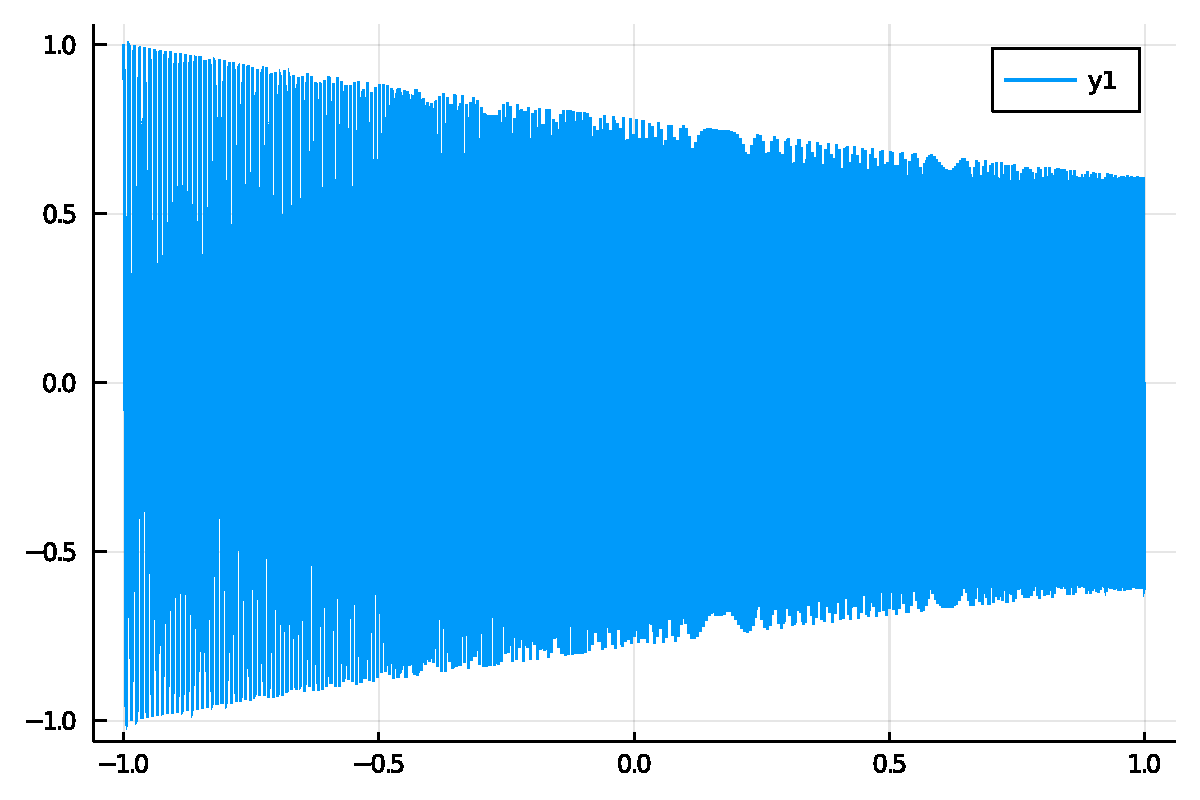
\includegraphics[width=0.9\linewidth]{C:/Users/mfaso/OneDrive/Documents/GitHub/M3M6AppliedComplexAnalysis/output/figures/Lecture20_20_1.pdf}}

\section{Differential equations satisfied by orthogonal polynomials}
Here we do the following:

\begin{itemize}
\item[1. ] Differential equations for orthogonal polynomials

\begin{itemize}
\item Sturm\ensuremath{\endash}Liouville equations


\item Weighted differentiation for ultraspherical polynomials


\item Differential equation for ultraspherical polynomials

\end{itemize}

\item[2. ] Application: Eigenstates of Schrödinger operators with quadratic potentials

\end{itemize}
The three classical weights are (Hermite) $w(x) = \E^{-x^2}$, (Laguerre) $w_\alpha(x) = x^\alpha \E^{-x}$ and (Jacobi) $w_{\alpha,\beta}(x) = (1-x)^\alpha (1+x)^\beta$. Note all weights form a simple hierarchy: when differentiated, they give a linear polynomial times the previous weight in the hierarchy.  For Hermite,
\[
{\D \over \dx} w(x) = -2x w(x)
\]
for Laguerre,
\[
{\D \over \dx} w^{(\alpha)}(x) = (\alpha  - x) w^{(\alpha-1)}(x)
\]
and for Jacobi
\[
{\D \over \dx} w^{(\alpha,\beta)}(x) = (\beta(1-x) - \alpha(1+x)) w^{(\alpha-1,\beta-1)}(x)
\]
These relationships  lead to simple differential equations that have the classical orthogonal polynomials as eigenfunctions.

\subsubsection{Sturm\ensuremath{\endash}Liouville operator}
We first consider a simple class of operators that are self-adjoint:

\textbf{Proposition (Sturm\ensuremath{\endash}Liouville self-adjointness)} Consider the weighted inner product
\[
\ip<f,g>_w = \int_a^b f(x) g(x) w(x) \dx
\]
then for any continuously differentiable function $q(x)$ satisfying $q(a) = q(b) = 0$, the operator
\[
Lu = {1 \over w(x)} {\D \over \dx}\left[ q(x) {\D u\over \dx} \right]
\]
is self-adjoint in the sense
\[
\ip<L f,g>_w = \ip<f, Lg>_w
\]
\textbf{Proof} Simple integration by parts argument:


\begin{align*}
\ip<L f,g>_w &= \int_a^b {\D \over \dx}\left[ q(x) {\D u\over \dx}\right]  g(x)\dx \ccr
=  -\int_a^b q(x) {\D u\over \dx}    {\D g\over \dx} \dx =  \int_a^b   u(x)  {\D \over \dx} \left[ q(x) {\D g\over \dx}\right] \dx \ccr
=
 \int_a^b   u(x)  {1 \over w(x)} {\D \over \dx}\left[q(x) {\D g\over \dx}\right] w(x) \dx = \ip<f, Lg>_w
 \end{align*}
\ensuremath{\blacksquare}

We claim that the classical orthogonal polynomials are eigenfunctions of a Sturm\ensuremath{\endash}Liouville problem, that is, in each case there exists a $q(x)$ so that
\[
L p_n(x) = \lambda_n p_n(x)
\]
where $\lambda_n$ is the (real) eigenvalue. We will derive this for the ultraspherical polynomials.

\subsubsection{Weighted differentiation for ultraspherical polynomials}
We have already seen that Chebyshev and ultraspherical polynomials have simple expressions for derivatives where we decrement the degree and increment the parameter:
\begin{align*}
{\D \over \dx } T_n(x) = n U_{n-1}(x) &= n C_{n-1}^{(1)}(x) \\
{\D \over \dx } C_n^{(\lambda)}(x) & = 2 \lambda C_{n-1}^{(\lambda+1)}(x)
\end{align*}
In this section, we see that differentiating the weighted polynomials actually decrements the parameter and increments the degree:

\textbf{Proposition (weighted differentiation)}
\begin{align*}
{\D \over \dx }[\sqrt{1-x^2} U_n(x)] &= - {n+1 \over \sqrt{1-x^2}} T_{n+1}(x) \\
{\D \over \dx }[(1-x^2)^{\lambda-\half} C_n^{(\lambda)}(x)] & = -{(n+1) (n+2 \lambda-1) \over 2 (\lambda-1) }  (1-x^2)^{\lambda - {3 \over 2}} C_{n+1}^{(\lambda-1)}(x)
\end{align*}
\newpage
\textbf{Proof} We show the first result by showing that the left-hand side is orthogonal to all  polynomials of degree less than $n+1$ by integration by parts:

\[
\ip< \sqrt{1-x^2} {\D \over \dx }[\sqrt{1-x^2} U_n(x)], p_m(x)>_{\rm T} = -\int_{-1}^1 \sqrt{1-x^2} U_n(x) p_m' \dx =0
\]
Note that

\[
\sqrt{1-x^2} {\D \over \dx } \sqrt{1-x^2} f(x) = (1-x^2) f'(x) - x f(x)
\]
Thus we just have to verify the constant in front:

\[
\sqrt{1-x^2} {\D \over \dx }[\sqrt{1-x^2} U_n(x) = (-n -1) 2^n x^{n+1}
\]
The other ultraspherical polynomial follow similarly. \ensuremath{\blacksquare}
\newpage
\subsubsection{Eigenvalue equation for Ultraspherical polynomials}
Note that differentiating increments the parameter and decrements the degree while weight differentiation decrements the parameter and increments the degree. Therefore combining them brings us back to where we started.

In the case of Chebyshev polynomials, this gives us a Sturm\ensuremath{\endash}Liouville equation:

\[
\sqrt{1-x^2} {\D \over \dx} \sqrt{1-x^2} {\D T_n \over \dx} =
n \sqrt{1-x^2} {\D \over \dx} \sqrt{1-x^2} U_{n-1}(x) = -n^2 T_n(x)
\]
Note that the chain rule gives us a simple expression as

\[
(1-x^2) {\D^2 T_n \over \dx^2} -x {\D T_n \over \dx} = -n^2 T_n(x)
\]
Similarly,

\[
(1-x^2)^{\half - \lambda} {\D \over \dx}(1-x^2)^{\lambda + \half} {\D C_n^{(\lambda)} \over \dx} = -n (n+2 \lambda) C_n^{(\lambda)}(x)
\]
or in other words,

\[
(1-x^2) {\D^2 C_n^{(\lambda)} \over \dx^2} - (2\lambda+1) x {\D C_n^{(\lambda)} \over \dx}  = -{n (n+2 \lambda) \over 2\lambda}C_n^{(\lambda)}(x)
\]

}
\end{document}
